% 原始稿件使用 pdfLaTeX；中文稿使用 XeLaTeX 编译，因此移除 \pdfoutput 设置。

\documentclass[11pt]{article}
\usepackage[UTF8]{ctex}

% Change "review" to "final" to generate the final (sometimes called camera-ready) version.
% Change to "preprint" to generate a non-anonymous version with page numbers.
\usepackage[final]{acl}

% Standard package includes
\usepackage{latexsym}

% 中文稿使用 XeLaTeX 与 ctex，无需额外的 fontenc/inputenc 设置。

% This is not strictly necessary, and may be commented out,
% but it will improve the layout of the manuscript,
% and will typically save some space.
\usepackage{microtype}

% This is also not strictly necessary, and may be commented out.
% However, it will improve the aesthetics of text in
% the typewriter font.
\usepackage{inconsolata}

%Including images in your LaTeX document requires adding
%additional package(s)
\usepackage{graphicx}

\usepackage{latexsym}
\usepackage{tabularx} % \usepackage{arydshln}
\usepackage{booktabs}
\usepackage{multirow}
\usepackage{subfigure}
\usepackage{amsmath}
\usepackage{amssymb}
\usepackage{array}
\usepackage{bm}
\usepackage{xparse}
\usepackage{mathtools}
\usepackage{pifont}
\usepackage{enumitem}
\usepackage{tcolorbox}
\tcbuselibrary{breakable}
\usepackage{listings}
 
\usepackage{arydshln}
\usepackage{hyperref}

% If the title and author information does not fit in the area allocated, uncomment the following
%
%\setlength\titlebox{<dim>}
%
% and set <dim> to something 5cm or larger.

\title{从 Personalization 与 Proactivity 视角\\评估个性化 Tool-Augmented LLMs}

% Author information can be set in various styles:
% For several authors from the same institution:
% \author{Author 1 \and ... \and Author n \\
%         Address line \\ ... \\ Address line}
% if the names do not fit well on one line use
%         Author 1 \\ {\bf Author 2} \\ ... \\ {\bf Author n} \\
% For authors from different institutions:
% \author{Author 1 \\ Address line \\  ... \\ Address line
%         \And  ... \And
%         Author n \\ Address line \\ ... \\ Address line}
% To start a separate ``row'' of authors use \AND, as in
% \author{Author 1 \\ Address line \\  ... \\ Address line
%         \AND
%         Author 2 \\ Address line \\ ... \\ Address line \And
%         Author 3 \\ Address line \\ ... \\ Address line}

% \author{First Author \\
%   Affiliation / Address line 1 \\
%   Affiliation / Address line 2 \\
%   Affiliation / Address line 3 \\
%   \texttt{email@domain} \\\And
%   Second Author \\
%   Affiliation / Address line 1 \\
%   Affiliation / Address line 2 \\
%   Affiliation / Address line 3 \\
%   \texttt{email@domain} \\}


\author{
 \textbf{Yupu Hao\textsuperscript{1,2}},
 \textbf{Pengfei Cao\textsuperscript{1,2}},
 \textbf{Zhuoran Jin\textsuperscript{1,2}},
 \textbf{Huanxuan Liao\textsuperscript{1,2}},
\\
 \textbf{Yubo Chen\textsuperscript{1,2}},
 \textbf{Kang Liu\textsuperscript{1,2}},
 \textbf{Jun Zhao\textsuperscript{1,2}},
\\
 \textsuperscript{1}The Key Laboratory of Cognition and Decision Intelligence for Complex Systems, \\Institute of Automation, Chinese Academy of Sciences, Beijing, China\\
 \textsuperscript{2}School of Artificial Intelligence, University of Chinese Academy of Sciences, Beijing, China
\\
\{haoyupu2023, liaohuanxuan2023\}@ia.ac.cn, \\ \{pengfei.cao, zhuoran.jin, yubo.chen, kliu, jzhao\}@nlpr.ia.ac.cn
 % \small{
 %   \textbf{Correspondence:} \href{mailto:email@domain}{email@domain}
 % }
}

\begin{document}
\maketitle
\begin{abstract}
个性化 tool utilization 对于在多工具交互场景中使 large language models（LLMs）与 user preference 对齐至关重要。然而，现有大多数 benchmark 主要聚焦于文本生成的个性化，或直接评测 tool-utilizing，而没有同时兼顾这两者。在这项工作中，我们提出一个新的 benchmark \textbf{ETAPP}，用于评测个性化 tool invocation，并构建了一个 sandbox environment 和一个覆盖多样化 user profile 的 800 条测试样例数据集。为提升评测准确性，我们提出一种基于 key point 的 LLM evaluation 方法：通过为每个测试样例人工标注 key point，并将其作为参考提供给 LLM，来缓解 LLM-as-a-judge 系统中的偏差。此外，我们对当前表现优异的 LLMs 进行了评测并给出深入分析。进一步地，我们研究了不同 tool-invoking strategy 对 LLM 个性化表现的影响，以及 fine-tuning 在本任务中的效果。我们还验证了所设计的 preference setting 与基于 key point 的评测方法的有效性。我们的发现为改进个性化 LLM agents 提供了启示。代码已开源于 \url{https://github.com/hypasd-art/ETAPP}。


\end{abstract}

\section{Introduction}
随着 large language model（LLM）能力的持续发展 \cite{zhao2024surveylargelanguagemodels}，越来越多的研究者开始将 alignment 的目标，从面向一般人群转向面向特定小群体甚至个体 \cite{chen2024personapersonalizationsurveyroleplaying, jang2023personalized}。LLM 的个性化，指的是调整 LLM 的行为与输出，使其更好地匹配个体用户的需求。在这一背景下，\citeauthor{li2024personalllmagentsinsights}\shortcite{li2024personalllmagentsinsights} 提出了 \textit{Personal LLM Agents} 的概念，即整合个性化用户数据与用户设备，为用户提供全面、连续且个性化的服务。为了实现这一目标，Personal LLM Agents 必须具备两项关键能力：memory \cite{zhang2024surveymemorymechanismlarge} 与 interaction \cite{10.1145/3704435, mialon2023augmentedlanguagemodelssurvey}。其中，memory 能力使模型能够追踪并保留用户的当前状态与历史信息，从而实现更具个性化且上下文感知的交互；而 interaction 能力则使模型能够与外部系统和设备交互，利用工具执行任务，并实时支持用户需求 \cite{li-etal-2023-api, DBLP:conf/iclr/QinLYZYLLCTQZHT24}。




当前，对 Personal LLM Agent 的评测主要仍聚焦于文本生成 \cite{zhao2025do}，对外部交互能力的关注相对有限。只有少量近期工作开始在涉及 tool utilization 的交互场景中评估 Personal LLM Agents。例如，\citeauthor{wang2024aipersonalifelongpersonalization}\shortcite{wang2024aipersonalifelongpersonalization} 构建了一个 life-long personal agent framework，并利用 LLM 对其进行评测。尽管该工作通过模拟外部 API 执行纳入了 tool calling，但并未专门评估交互过程本身。\citeauthor{cai2024largelanguagemodelsempowered}\shortcite{cai2024largelanguagemodelsempowered} 则在 online shopping 这一特定领域、使用有限工具集评估了个性化 tool usage。然而，这些工作仍未回答以下两个核心问题：(1) 与普通的 tool-utilizing 相比，应当设计怎样的评测指标来衡量 personalized tool-utilizing？(2) 我们该如何在更真实的环境中，而非局限于狭窄领域与模拟场景中，有效评估个性化 tool usage 能力？





\begin{figure*}[t]
  \centering
  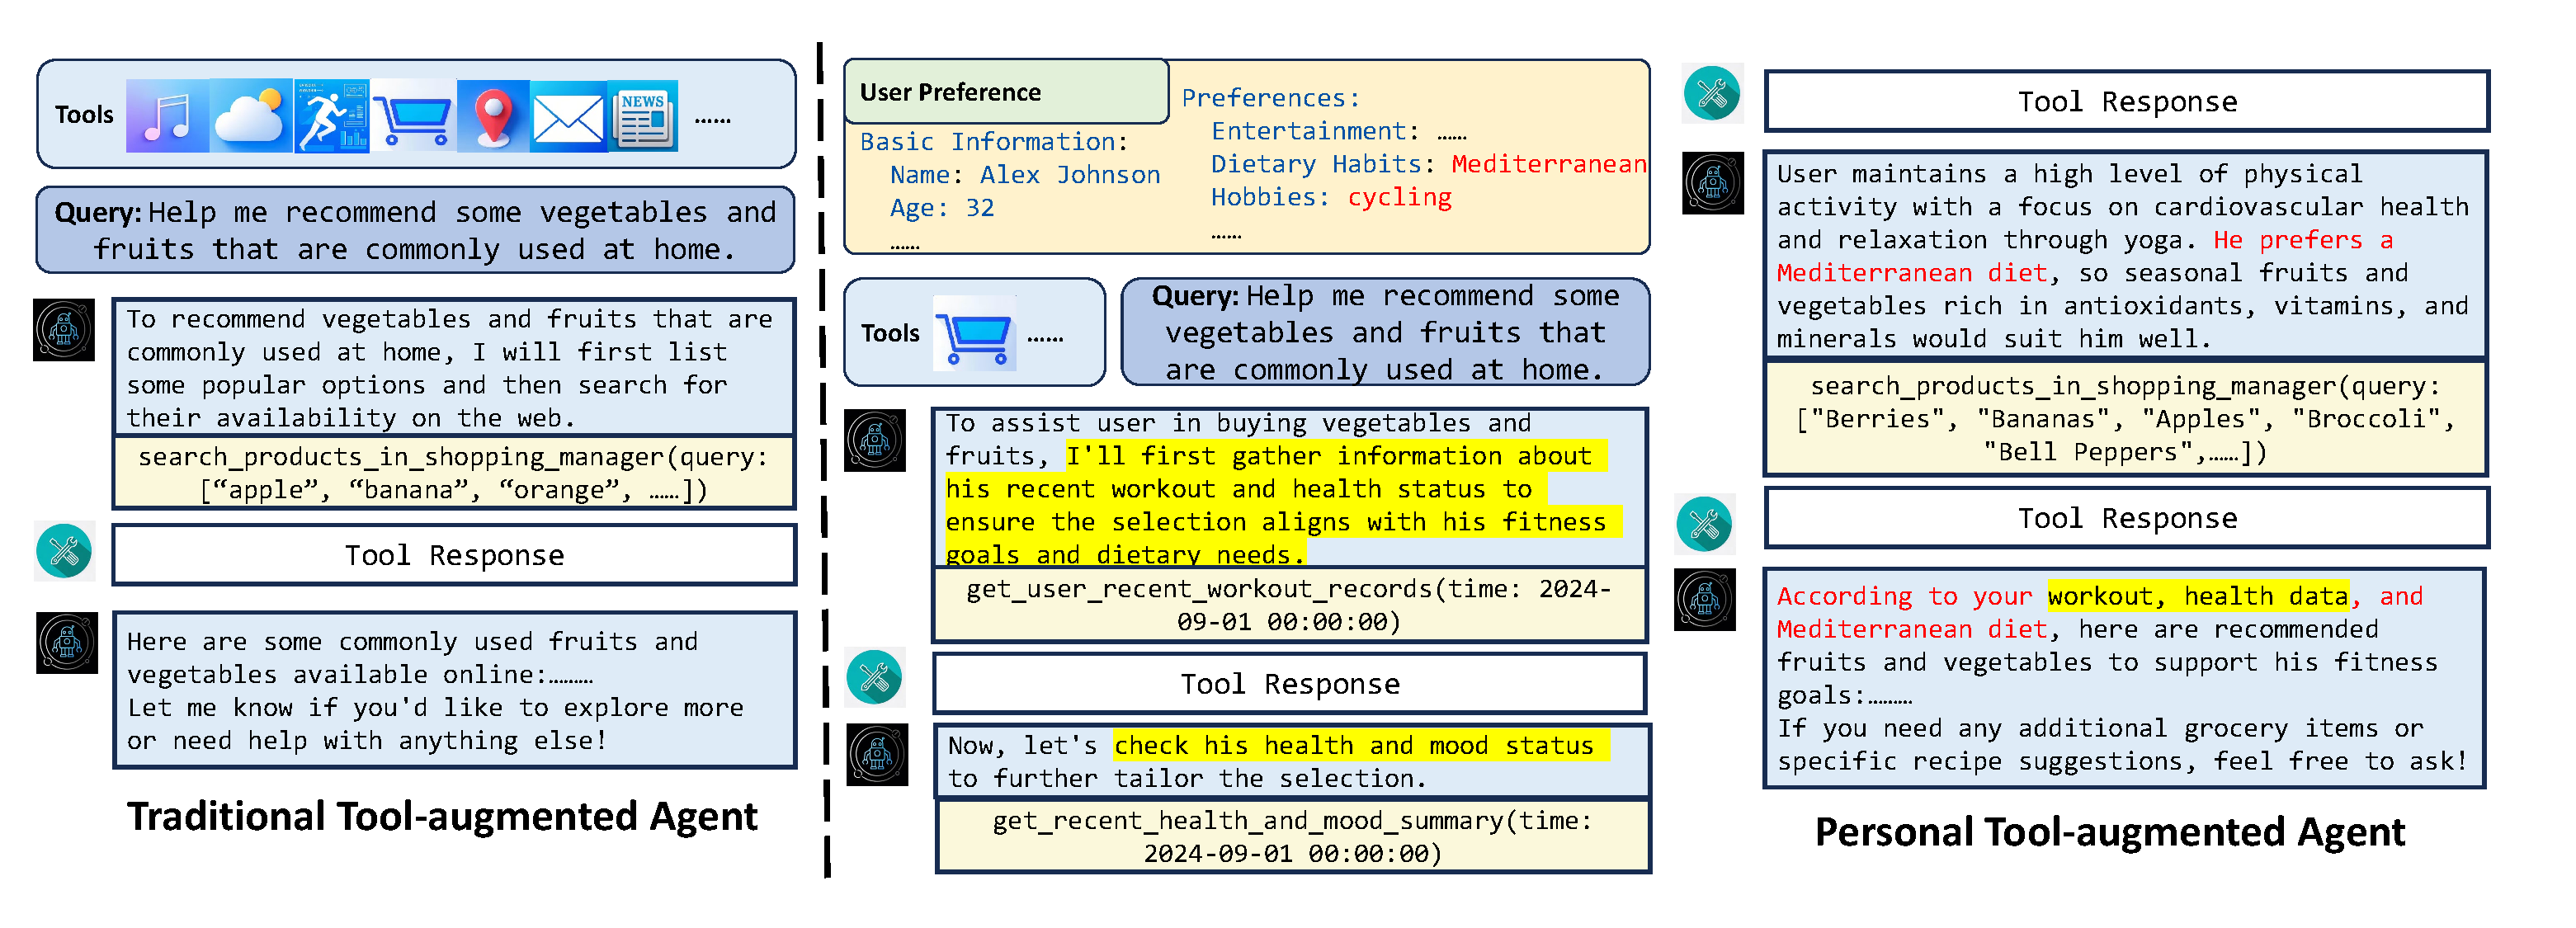
\includegraphics[width=0.95\textwidth]{pic/different_model.pdf} 
  \caption{传统 tool-augmented agent 与 personal tool-augmented agent 的差异。红色字体表示体现 personalization 的输出，黄色背景字体表示体现 proactivity 的输出。
  }
    \label{fig:different_model}
\end{figure*}

为回答第一个问题，我们认为，理想的 personal assistant 不仅应当提供个性化服务，还应理解用户意图并预判其未明说的需求。它应当考虑即时指令之外的因素，提供更全面的支持，以减轻用户负担。从这一视角出发，图~\ref{fig:different_model} 展示了传统 tool-augmented LLM 与 personal tool-augmented LLM 之间的差异。后者应当体现两个关键特征：personalization 与 proactivity。 \textbf{Personalization} 要求模型根据用户的偏好与需求来定制其响应与工具使用方式。例如，当用户请求食物推荐时，个性化 LLM 会考虑用户偏好 Mediterranean diet（图中红字部分），而传统 agent 往往只会给出热门选项。 \textbf{Proactivity} 则指模型能够超出用户显式请求，主动预判并建议额外行动，从而更完整地帮助用户完成任务。例如，assistant 会进一步查看用户近期的健康状态与锻炼记录，以定制更贴合的推荐（图中黄色背景部分）；而传统模型通常会忽略这些因素。这一行为并非用户明确要求，但能够有效提升服务质量。







基于上述两个指标，我们构建了一个新的 benchmark，称为 \textbf{E}valuation of \textbf{T}ool-augmented \textbf{A}gent from the \textbf{P}ersonalization and \textbf{P}roactivity Perspective（\textbf{ETAPP}），用于评估 large language models 的个性化 tool invocation 能力。对于该 tool-invoking framework，我们构建了一个简洁的 sandbox，以保证测试过程的稳定性，其关键组成包括：(1) Environment Setup：我们开发了一个包含 33 个 functional API（如 \textit{add\_calendar}、\textit{view\_calendar}、\textit{get\_weather}）的 tool-invoking system，这些 API 隶属于 9 个类别（如 \textit{Calendar}、\textit{Weather}），覆盖软件 API 与硬件 API。为提升评测的真实性与稳定性，我们设计了一个简单的 sandbox environment，使 API 响应不受外部环境变化影响。(2) Memory Building：personal LLM agents 的 memory 包括长期用户偏好与短期用户状态。我们将用户偏好划分为两类：高层 user profile 与底层 tool-utilizing preference，以便更精确地捕捉用户需求。我们基于职业背景生成了 16 种不同 user profile，作为构建多样化评测样本的基础。为模拟真实使用场景，我们还为每个必要工具与每位用户构建了 9 天的 interaction history。(3) Instruction Construction：我们人工标注了 50 条测试指令，并将其与 16 种不同 user profile 组合，得到最终包含 800 条测试样例的数据集。该数据支持我们从 personalization 与 proactivity 两个角度评估个性化 tool invocation 能力。




为回答第二个问题，我们使用 LLM 作为评测模型，对 tool-invoking system 的表现进行打分 \cite{li2025generationjudgmentopportunitieschallenges, li2024llmsasjudgescomprehensivesurveyllmbased}。为了提升评测可靠性，我们设计了一种基于 key point 的 LLM evaluation 方法。每条测试指令都对应若干由人工标注的 key point，它们作为任务完成情况的标准指示器提供给 evaluation LLM 以辅助评分。评测模型首先判断每个要点是否被满足，再给出最终分析与分数。实验结果表明，这些 key point 能够显著提升评测准确性。






最后，我们在完整测试集上评估了当前具备 tool invocation 能力的优秀 LLMs，并在测试子集上评估了一些 reasoning models（如 o1-mini、DeepSeek-R1）。结果表明，LLMs 往往倾向于直接回答问题，而没有深入推理“为什么要选择这个工具”，或者对个性化 tool-utilizing 过程考虑不足。进一步地，我们分析了不同 tool-invoking method 对性能的影响，结果指出 reasoning process 在 tool-utilizing 中的重要性。此外，我们还人工标注了部分测试数据，并使用这些数据对一个 7B 模型进行 fine-tuning。结果显示，fine-tuning 能够提升模型在 in-domain instruction data 上的表现，但对 out-of-domain instruction data 的作用有限。






总的来说，我们的贡献包括：
\begin{itemize}
    \item 我们开发了一个用于个性化 tool invocation 的新 benchmark，并建立了一个稳定一致的 sandbox environment 用于评测。基于包含 800 条测试样例、覆盖多种 user profile 与 preference 的数据集，我们从 personalization 与 proactivity 两个视角评估模型表现。
    \item 我们提出了一种基于 key point 的 LLM evaluation 方法，通过对每条测试数据人工标注 key point 来辅助评测，相比直接评测提高了可靠性。
    \item 我们专门验证了所设计 preference 方案与评测方法的有效性，并分析了不同 tool-invoking method 的影响，以及 fine-tuning 在不同场景下如何影响模型性能。
\end{itemize}





\section{Dataset Construction}
如图~\ref{fig:process_construction_dataset} 所示，该构建流程包括以下组成部分：Environment Setup、Memory Building 与 Instruction Construction。



\subsection{Environment Setup}
为了更好地模拟真实世界应用场景，我们手工构建了一个 tool-invoking environment，其中包含 33 个 functional API（如 \textit{add\_calendar}、\textit{get\_weather}），隶属于 9 个类别，以及 2 个用于搜索可用工具的 tool retrieval API（\textit{search\_tools} 和 \textit{get\_tool\_doc}）。这些 API 覆盖了广泛的常见软件 API（如 Calendar 与 Email）以及依赖硬件的 API（如通过智能手环进行 health monitoring，以及 smart home control），从而保证了足够广泛的实际使用场景。



此外，我们还开发了一个简单的 sandbox environment，以确保测试过程的稳定性与可靠性。该 sandbox 将实验与外部环境变量（如 connection error 或外部世界状态变化）隔离开来，从而避免 API 输出受到外部因素影响，并保证评测的准确性。我们使用真实世界的 API 数据来生成相应输出（例如来自 RapidAPI 的数据），以增强模拟场景的真实性。更多细节请参见 Appendix~\ref{sec:dataset_construction}。




\begin{figure}[t]
  \centering
  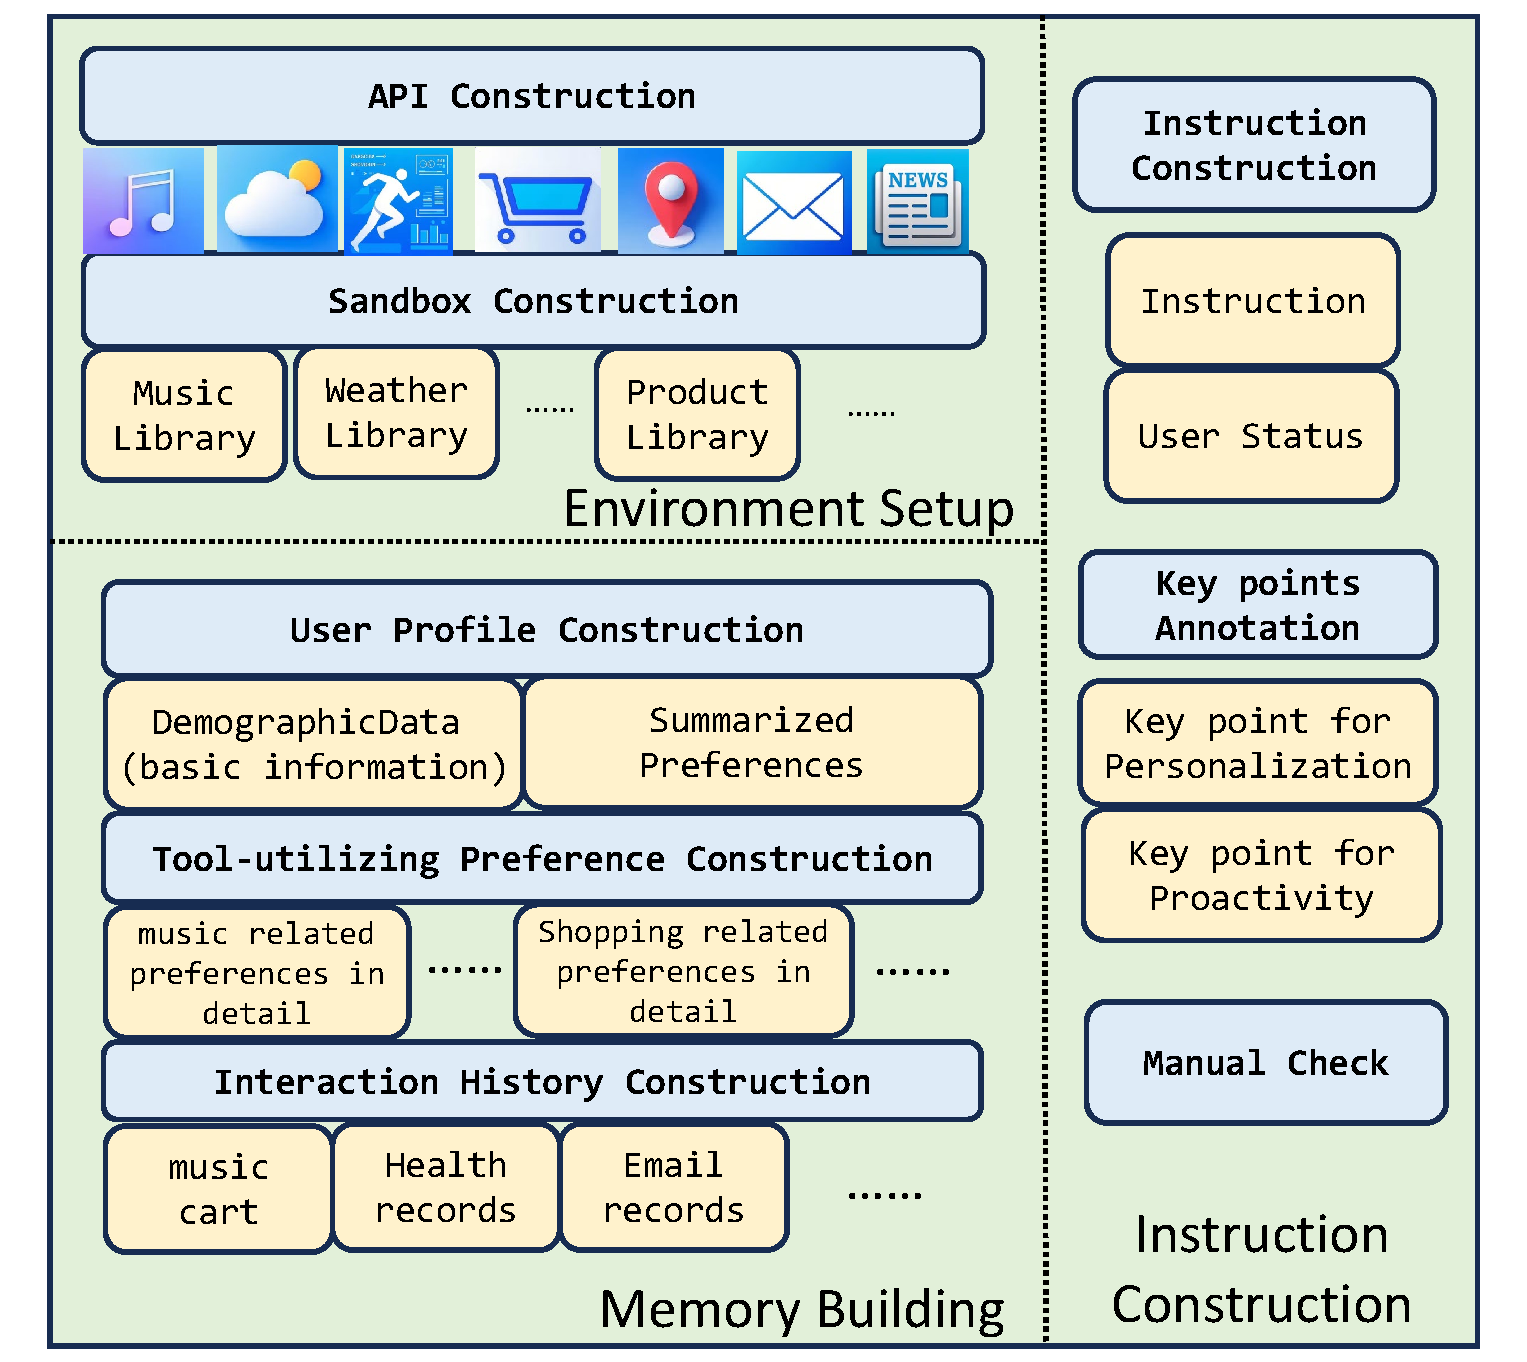
\includegraphics[width=\columnwidth]{pic/construct_dataset.pdf} 
  \caption{数据集构建流程。
  }
    \label{fig:process_construction_dataset}
\end{figure}





\subsection{Memory Building}
LLM 个性化的核心在于有效利用用户 memory，而这类 memory 可以分为 long-term memory（捕捉用户的偏好、习惯与历史行为）和 short-term memory（反映用户当前状态，例如位置）。

\subsubsection{Long-term and Short-term Memory}
对于 long-term memory，我们提出了一种新的架构，将用户偏好进一步细分为两类，以更有效地管理 memory：\textbf{high-level preferences}（User Profile）与 \textbf{low-level preferences}（Tool-utilizing Preference）。User Profile 包含用户的基本信息（如姓名、年龄与职业）以及对其偏好的概述性描述；而 Tool-utilizing Preference 则包含用户在对应类别 API 上的详细偏好描述。例如，对于 music 类 API，我们建立了一套统一的 music-utilizing preference，其中包括喜欢的音乐、歌手、收听习惯等属性，从而为模型调用相应工具并生成响应提供更细粒度的指导。我们为每位用户建立了 8 类 tool-utilizing preferences（\textit{Weather} 类别未设计偏好）。当对应工具被调用时，相关类别的 preference 会预先输入模型，作为上下文信息以辅助模型生成个性化输出。

由于用户数据量庞大且 context window 有限，一次性输入全部 preferences 既不现实也不高效。传统方法 \cite{zhao2025do} 通常从 dialogue history 中总结 preference，但这种方式往往覆盖稀疏且不完整，有些偏好甚至不会在对话中体现出来。相比之下，从 API 视角总结 preference 更加全面，也更准确。



具体而言，我们借助 LLM 完成如下 memory construction 过程。首先，LLM 基于不同职业生成 16 种不同的 user profile。随后对这些 profile 进行人工校验，以确保其在多样性与一致性上都达到要求，并覆盖广泛的用户类型。其次，在上述 profile 基础上，LLM 进一步为每位用户生成 8 类 tool-utilizing preference，之后同样经过人工验证，以确保其相关性与准确性。


对于 short-term memory，我们为每条测试数据定义用户当前状态，包括 location 与 current time，以更准确地反映用户的个性化需求。


\subsubsection{Interaction History Construction}
需要指出的是，一些工具依赖用户的 interaction history（例如检索近期锻炼记录或邮件记录）。因此，我们需要为特定 API 构建 interaction history。

为了确保 interaction history 的一致性，我们首先为每位用户构建一个 9 天安排，并在其基础上生成 interaction history，覆盖日程安排、闹钟、健康状态（按小时更新）、锻炼记录、邮件记录和音乐收藏。具体步骤见 Appendix~\ref{sec:appendix_instruction_history}。








\subsection{Instruction Construction}
\label{sec:instruction_construction}
我们人工标注了 50 条独立 instruction，并将其与 16 个预定义 user profile 组合，共构成 800 条测试 instruction。对于每条 instruction，我们都提供用户状态（即用户的当前时间与位置）。为了保证 interaction history 的准确性并避免潜在冲突，我们再次核验了这 9 天 interaction history，以确保每条 instruction 都能在环境中得到回答。此外，我们还为每条 instruction 人工编写了 key points。我们将这些 key points 定义为：在预定义环境中，为实现 personalization 与 proactivity 而必须满足的具体要求。这些 key points 被用于 Section~\ref{sec:evaluation_framework} 中的评测。数据集统计信息见 Table~\ref{table:statistics}。





\begin{figure*}[t]
  \centering
  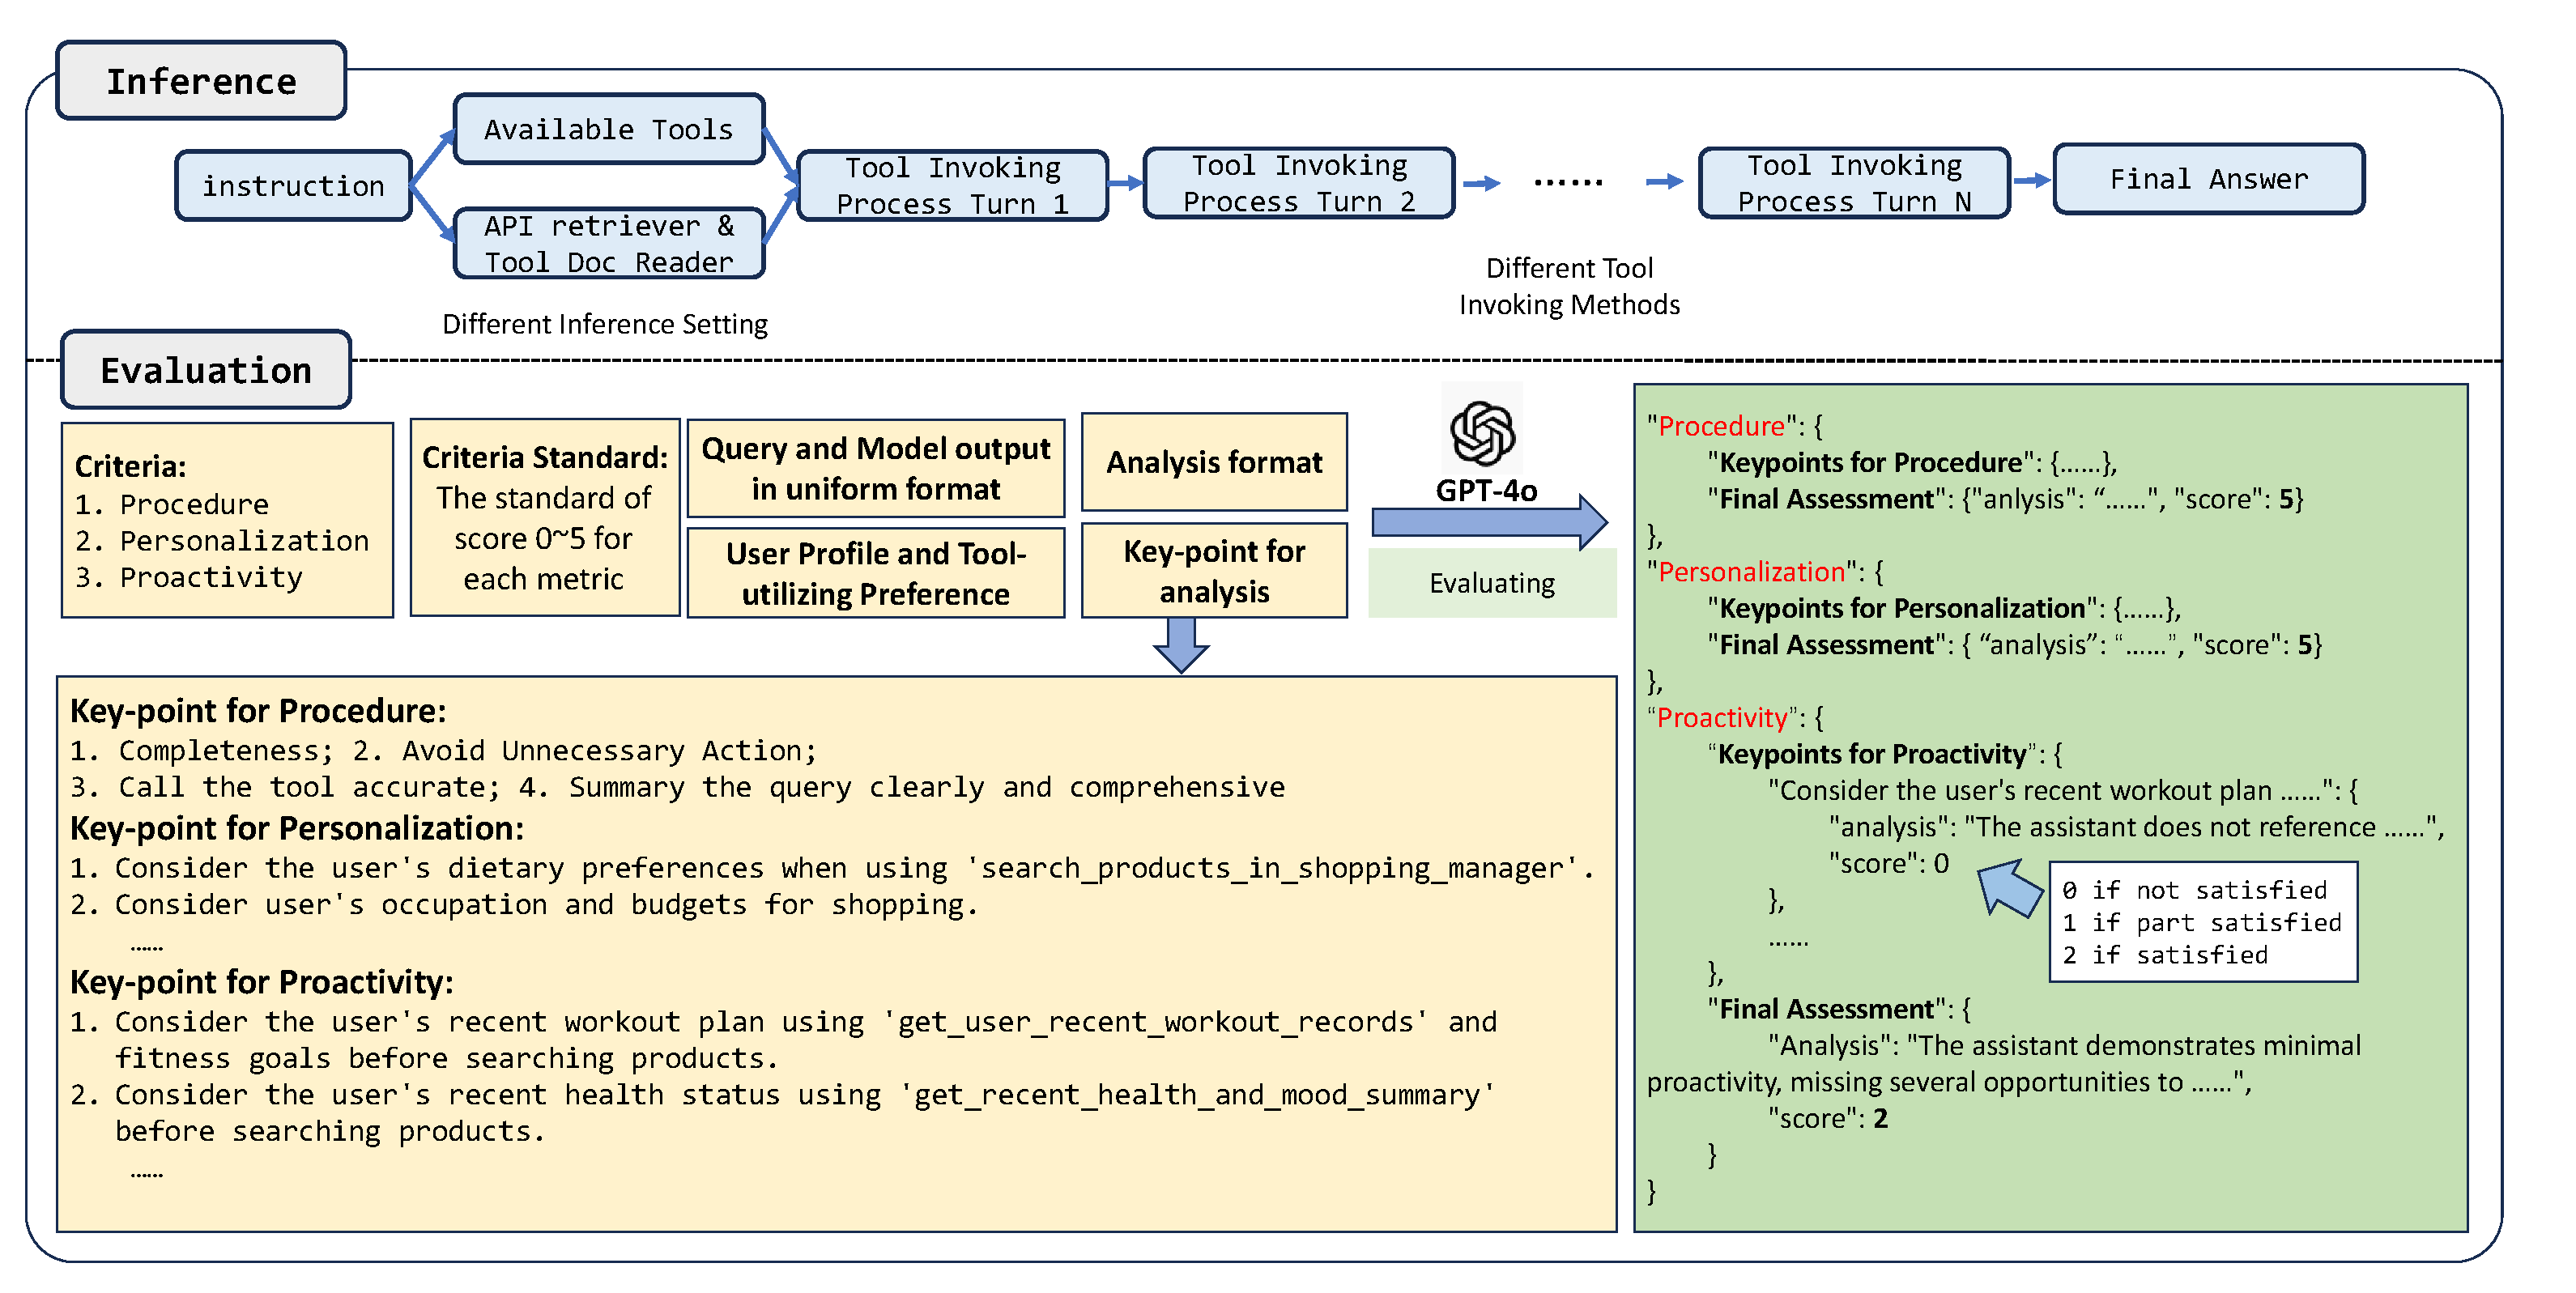
\includegraphics[width=\textwidth]{pic/model_arc.pdf} 
  \caption{我们 benchmark 的 Inference 与 Evaluation 流程。
  }
    \label{fig:process}
\end{figure*}
\section{Evaluation}
\subsection{Evaluation Metrics}
评测过程使用 large language model 进行打分，评分标准基于三个维度，每个维度的分值范围均为 0 到 5：
(1) \textbf{Procedure (PRC)}：该指标评估模型是否给出了完整且准确的最终响应。评分依据是模型是否覆盖了用户 query 的全部关键方面，并在没有遗漏的情况下给出清晰、全面的解决方案。
(2) \textbf{Personalization (PSN)}：该指标评估模型是否恰当地将用户偏好与当前状态融入响应之中，是否能够根据用户历史数据与需求定制其解决方案。
(3) \textbf{Proactivity (PTV)}：该指标衡量模型是否超越了用户的显式指令，通过采取额外且有意义的步骤来更有效地帮助用户，能否主动识别用户需求并提供额外建议或行动，而不是仅仅被动响应用户请求。






\subsection{Evaluation Settings}
评测包含两种 evaluation setting：
(1) \textbf{Tool-Given}：在该设定下，工具是预先给定的，评测重点在于模型能否借助已知工具有效完成任务。
(2) \textbf{Tool-Retrieval}：该设定更接近真实世界场景。模型需要在有限 context window 内，根据任务需求搜索工具及其对应的 utilizing preference，并调用它们完成任务。


基于上述数据与方法，我们构建了一个完整的 Inference framework，如图~\ref{fig:process} 所示。该框架包含以下组成：对于用户 $u$ 与 instruction $Q$，输入包括 system prompt $I$、可用工具 $T_Q$、用户高层 profile preference $P_h^u$、用户 tool-utilizing preference $\{P_t^u|t \in T_Q\}$、用户状态 $C_Q^u$ 以及 one-shot example（可选）$E$。这些元素共同作为模型输入，模型输出则是某次 tool invocation 或最终响应。LLM 通过与工具交互来处理 instruction，并在获得最终结果或达到预定义最大步数后终止。




在 Tool-Given 与 Tool-Retrieval 设定下，该过程分别可形式化表示如下：



\begin{equation}
\footnotesize
\begin{aligned}
    A_n&:\text{Tool\_Given} = LLM(I, T_Q^u, P_h^u, \{P_t^u|t \in T_Q\}, \\ &C_Q^u, E, Q, \sum_{i=1}^{n-1}(A_i, O_i))\\
    A_n&:\text{Tool\_Retrieval} = LLM(I, T_Q^u, P_h^u, C_Q^u, E, Q, \\ &\sum_{i=1}^{n-1}(A_i, O_i, \{P_t^u|t \in o_i^j \text{ and } a_i^j=\text{tool\_search}\}))
\end{aligned}
\end{equation}


其中，在步骤 $i$ 上，$A_i$ 表示 LLM 的输出，$a_i^j$ 表示 $A_i$ 中第 $j$ 次 tool calling，$O_i$ 表示对应工具的 observation。







\subsection{Evaluation Framework}
\label{sec:evaluation_framework}
我们提出了 key-point-based LLM evaluation framework。由于解题路径并不唯一，而 preference evaluation 又具有多维性与较高难度，现有方法通常在评测 tool utilizing ability \cite{DBLP:conf/iclr/QinLYZYLLCTQZHT24} 或 preference alignment \cite{zhao2025do} 时使用 LLM 作为 evaluator。然而我们发现，直接评估 LLM 表现是困难的，因为评测模型对 personalization 与 proactivity 的理解有限，难以准确判断输出是否达到要求。为改善这一点，我们需要促使 evaluation model $E\_LLM$ 从更具体的方面分析模型输出，因此我们向 evaluation LLM 提供人工编写的 key points。






如图~\ref{fig:process} 所示，对于每条 instruction $Q$ 和用户 $u$，0 $\sim$ 5 分的评分标准会在 system prompt $I_E$ 中提供给评测模型。与此同时，用户 profile preference、tool-utilizing preferences 以及被评测模型的输出也会输入给 evaluation model。此外，我们还提供每个指标对应的 key points $K$ 以及输出分析格式 $F$。评测模型会对每个 key point 给出分析与分数（0 $\sim$ 2），并进一步给出该 instruction 上模型表现的最终得分。形式化表示如下：


\begin{equation}
\footnotesize
\begin{aligned}
    & \text{Analysis}, \text{Score} = E\_LLM(Q, I_E, P_h^u, \\ &\{P_t^u|t \in T_Q\}, \sum_{i=1}^{N}(A_i, O_i), K, F)
\end{aligned}
\end{equation}






\begin{table*}[t]
\centering
{
    
	\centering
    \resizebox{1\textwidth}{!}{
	\begin{tabular}{l | c | c c c | c  c  c | c } %
        \hline
		% \toprule
        
        
        \multirow{2}{*}{\textbf{Model}} 
        & \multirow{2}{*}{\textbf{Method}}
        & \multicolumn{3}{c|}{\textbf{Tool Given}}
        & \multicolumn{3}{c|}{\textbf{Tool Retrieval}}
        & \multirow{2}{*}{\textbf{Average}}
        \\

		
		&
		& \textbf{PRC}
		& \textbf{PSN}
        & \textbf{PTV}
        & \textbf{PRC}
		& \textbf{PSN}
        & \textbf{PTV}
        &
        \\
		\midrule
        
        
        GPT-4o
        & \multirow{5}{*}{\textbf{FC}}
		& \textbf{3.95} 
		& \textbf{3.37} 
        & \textbf{1.61}
        & 2.67
        & 2.19
        & \textbf{1.08}
        & \textbf{2.48}
        
		\\
        % \cline{1-1}
        % \cline{3-9}
        % \midrule
  
		DeepSeek-V3
        &
		& 3.02 
        & 2.78 
        & 1.47
        & 2.57
        & \textbf{2.38}
        & 0.95 
        & 2.20

        \\
        % \cline{1-1}
        % \cline{3-9}
        % \midrule

        
        Llama-3.1-70B-Instruct
        &
		& 2.31 
        & 1.71 
        & 0.55
        & 1.50
        & 1.06
        & 0.30
        & 1.24

        \\
        % \cline{1-1}
        % \cline{3-9}
        % \midrule


        Qwen2.5-72B-Instruct
        &
		& 3.76 
		& 3.34 
        & 1.5 
        & \textbf{2.72} 
        & 2.31 
        & 1.05
        & 2.45
        
        \\
        % \cline{1-1}
        % \cline{3-9}
        % \midrule
        
        
        watt-tool-70B
        &
		& 2.70 
		& 1.97 
        & 0.71
        & 0.84
        & 0.32
        & 0.12
        & 1.11
        
		\\
        \hline
        \hline
        % \midrule
        % \midrule

        GPT-4o
        & \multirow{7}{*}{\textbf{ReAct}}
		& 3.97 
		& 3.61 
        & 1.60
        & 3.70
        & 3.43
        & 1.56
        & 2.98
        
		\\
        % \cline{1-1}
        % \cline{3-9}
        % \midrule
  
		DeepSeek-V3
        &
		& \textbf{4.05} 
        & \textbf{3.78}
        & 1.84
        & \textbf{3.82}
        & \textbf{3.54}
        & \textbf{1.65} 
        & \textbf{3.11}

        \\
        % \cline{1-1}
        % \cline{3-9}
        % \midrule

        o1-preview *
        &
		& 3.67 
		& 3.69 
        & \textbf{1.87}
        & 3.28
        & 3.48
        & 1.60
        & 2.93
        
		\\
        % \cline{1-1}
        % \cline{3-9}
        % \midrule
  
		o1-mini *
        &
		& 3.63 
        & 3.35 
        & 1.61
        & 3.25
        & 3.14
        & 1.35 
        & 2.72

        \\
        % \cline{1-1}
        % \cline{3-9}
        % \midrule

        
        DeepSeek-R1 *
        &
		& 2.41 
        & 2.06 
        & 1.35
        & 0.93
        & 0.40
        & 0.31
        & 1.24

        \\
        % \cline{1-1}
        % \cline{3-9}
        % \midrule


        DeepSeek-R1-Distill-Qwen-32B *
        &
		& 2.40 
		& 2.57 
        & 1.07 
        & 1.74 
        & 1.66 
        & 0.62
        & 1.68
        
        \\
        % \cline{1-1}
        % \cline{3-9}
        % \midrule
        
        
        QwQ-32B-Preview *
        &
		& 1.01 
		& 1.19 
        & 0.53
        & 0.61
        & 0.48
        & 0.18
        & 0.67
        
		\\
        \hline
        % \midrule



		% \bottomrule
	\end{tabular}
}
}
	\caption{不同 LLMs 在两种设定下的整体结果。* 表示仅在子集数据上测试。我们使用的 evaluation model 为 GPT-4o。
	}
	\label{table:overall_result}
\end{table*}











\section{Experiments}
\subsection{Baselines}
我们采用两种常用的 tool-invoking method：\textbf{FC (Function Calling)}：模型在 fine-tuning 后通过预定义格式调用工具；\textbf{ReAct} \cite{yao2023react}：模型将 reasoning 与 tool invocation 结合，其中 reasoning 引导模型分析当前状态并决定合适的 action。在该过程中，我们为 ReAct 提供 one-shot example。





在两种实验设定下，我们选用具备 function calling 能力的优秀 closed-source 与 open-source 模型作为 baselines。此外，由于 budget 因素，我们使用 ReAct method 在 100 条测试数据的子集上评估 reasoning model，因为这些模型不支持 FC。更多细节请参见 Appendix~\ref{sec:evaluation_details}。




\subsection{Evaluation Results}
结果如 Table~\ref{table:overall_result} 所示。我们可以在 FC 结果中观察到：(1) 在 Tool-Retrieval 场景下，模型表现显著低于 Tool-Given 场景，这表明随着 tool-invoking 与 planning 长度和难度的上升，模型面临更大挑战；(2) 在当前 FC 设定下，GPT-4o 在多个指标上表现优秀，而 Qwen2.5-72B-Instruct 优于 DeepSeek-V3，体现出较强性能；(3) 即便是在 BFCL \cite{berkeley-function-calling-leaderboard} 中表现最好的模型 Watt-tool-70B，在本 tool-invoking 任务上也存在明显困难。这可能有两个原因：a) 泛化能力不足。post-training 可能削弱了它在 tool-planning 过程中充分把握 personalization 与 proactivity 的能力；b) 缺乏深度推理。在工具学习过程中，模型倾向于依据显式指令直接调用工具，而不是进行深入推理，因而难以有效处理缺少明确指令的 Proactivity 场景。这启发我们，除了提升模型“会用工具”的能力，还要提升其“为什么调用这个工具”的思考能力。


reasoning models 在本任务中并未体现出相对于非 reasoning 模型的优势，尤其是 DeepSeek-Distill 与 QwQ 模型，其表现较差。这可能说明 reasoning model 并未将 reasoning process 与 tool-invoking process 有效整合，或者在特定场景中没有围绕 Personalization 与 Proactivity 进行足够深入的思考。一些错误样例可见 Appendix~\ref{sec:appendix_example_error}。


\begin{figure*}[t]
  \centering
  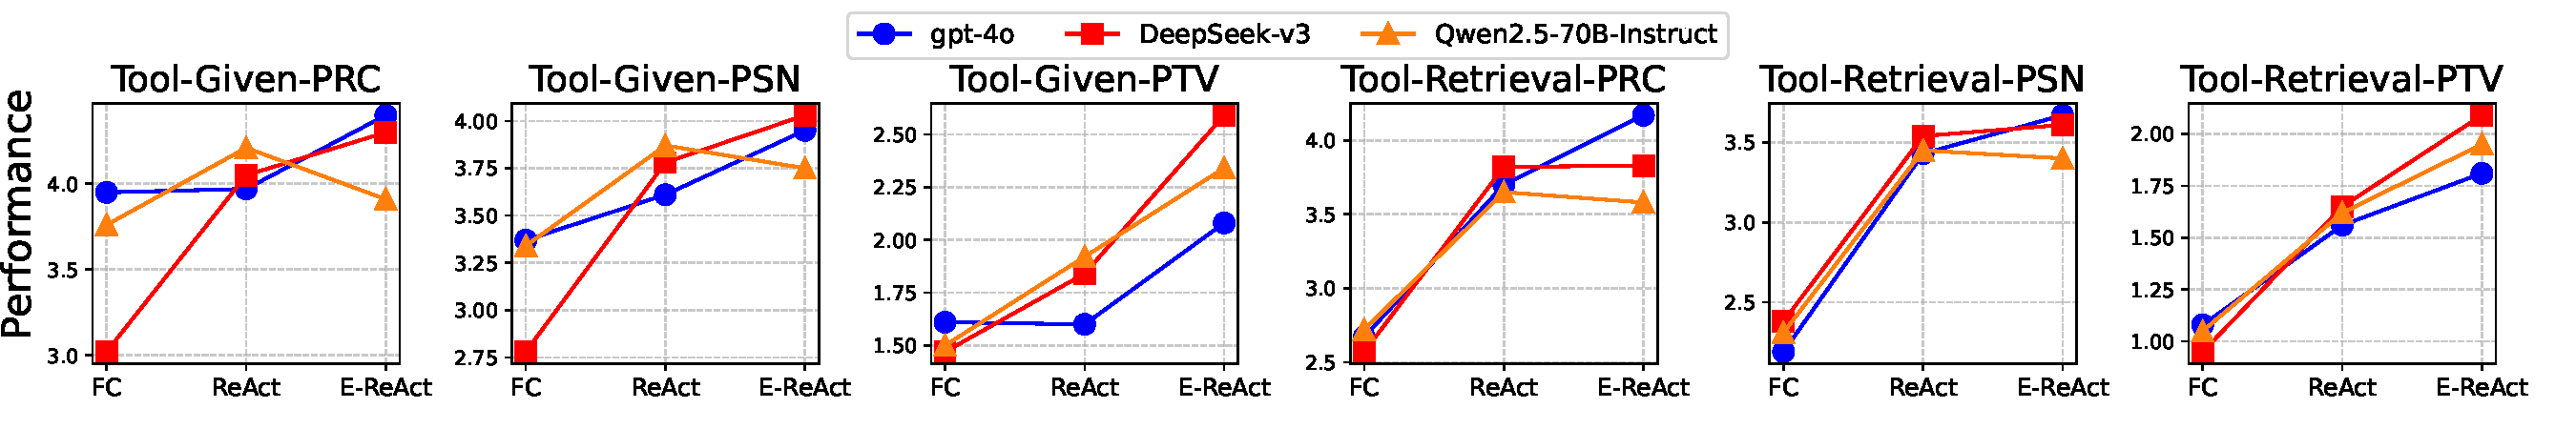
\includegraphics[width=\textwidth]{pic/inference.pdf} 
  \caption{不同 tool-invoking methods 的性能。
  }
    \label{fig:different_inference_performance}
\end{figure*}

\subsection{Analysis}
\subsubsection{Tool-invoking Method Analysis}
为了分析不同 tool-invoking method 对模型性能的影响，我们采用以下三种方法：\textbf{FC}、\textbf{ReAct} 和 \textbf{E-ReAct (Enhanced-ReAct)}。E-ReAct 在 ReAct 基础上进行了扩展：在调用工具之前，先要求模型生成 personalization 与 proactivity 的关键方面；在明确这些关键点之后，再使用 ReAct 框架进行 tool invocation，以完成任务。




如 Figure~\ref{fig:different_inference_performance} 所示，我们发现 E-ReAct 方法能够有效提升模型输出在 personalization 与 proactivity 方面的能力。通过在 tool invocation 之前引入强制性的深度思考与理解过程，模型能够更好地解释用户意图，并提供更主动的服务。这表明，在 tool-learning 过程中融入更多高质量 reasoning，可能会带来更好的性能。



\begin{table}[]
    \centering
    \resizebox{0.9\columnwidth}{!}{
    \begin{tabular}{c|c|c|c|c}
        \midrule
        Setting & Tokens & PRC & PSN & PTV
        \\
        \hline
         All & 3444 &  4.09 & \textbf{3.80}  & 1.62 \\
         \hline
         Needed & \textbf{2393} & \textbf{4.16} & 3.73 & \textbf{1.76}
         \\
         \hline
    \end{tabular}}
    \caption{不同 preference setting 在子集数据上的评测结果。 \textit{Tokens} 指标表示由 Llama-3.1-70B-Instruct 的 tokenizer 计算得到的每条 instruction 的平均 token 数。性能测试模型为 GPT-4o。 
    }
    
    \label{table:different_preference_setting}
\end{table}
\subsubsection{Preference Setting Analysis}
我们将 preference 划分为 User Profile 与 Tool-utilizing Preference。Table~\ref{table:different_preference_setting} 展示了“将全部 preferences 输入 LLM”与“采用我们的方法”之间的差异。可以看到，我们的设定（Needed）缩短了 context length，并取得了与全部输入（All）相当甚至具有竞争力的结果。需要指出的是，我们目前只纳入了 8 个类别的 preferences；随着类别数量增加，或者 preference 变得更加细致，我们的方法优势预计会更加明显。


\subsubsection{Fine-tuning Experiments Analysis}
为了验证我们关于 reasoning 重要性的判断，我们分别标注了一部分 ReAct 格式和 FC 格式的数据，并使用 200 条数据在 Qwen2.5-7B-Instruct 上开展 fine-tuning experiments。标注流程如下：
(1) 使用 LLM 生成参考答案。
(2) 对答案进行人工核验与标注，以确保质量与一致性。
对于 FC 格式数据，其中一组仅包含 tool-calling process，而另一组还包含 tool invocation 之前的文本思考过程。

结果见 Table~\ref{table:fine-tuning-result}。我们发现：(1) 对于 ID instructions 和 OOD users，性能提升显著。然而，OOD instructions 的提升明显低于 ID instructions，这说明：对于同一场景内的 instruction，只要模型学会了 tool invocation process，即便用户偏好不同，它也能够泛化并解决问题；但当出现新场景时，模型难以有效推理“应当如何解决问题”，从而导致提升有限。(2) 与 ReAct 和 FC 模型相比，“wo r” 的提升并不显著，这表明要增强模型的多轮 tool invocation 能力，仍然需要一定程度的 reasoning process。(3) 与 FC 相比，ReAct 这类 tool-invoking method 在该模型上依然表现出优势。



\begin{table}[t]
\centering
% \setlength{\tabcolsep}{2pt}
{
   \renewcommand{\arraystretch}{0.9} 
	\centering
    \resizebox{1\columnwidth}{!}{
	\begin{tabular}{l | c c c } %
		\toprule
        
        
        \textbf{Model} 
        

		
		
		& \textbf{PRC}
		& \textbf{PSN}
        & \textbf{PTV}

        \\
		\midrule

        \multicolumn{4}{c}{\textbf{U(ID)I(OOD)}}
        \\
        \midrule
        \midrule
        
        
        Vanilla (ReACT)
		& 2.76 
		& 2.97 
        & 1.35
        
		\\
        % \midrule
  
		\quad FT (ReAct)
		& \textbf{3.47} ($\uparrow$ 25.8\%) 
        & \textbf{3.28} ($\uparrow$ 10.4\%) 
        & \textbf{1.99} ($\uparrow$ 47.4\%)

        \\
        \midrule
        % \midrule

        
        Vanilla (FC)
		& 3.08 
        & 2.66 
        & 1.07

        \\
        % \midrule


        \quad FT (FC)
		& 3.23 ($\uparrow$ 4.9\%) 
		& 3.00 ($\uparrow$ 12.8\%) 
        & 1.72 ($\uparrow$ 60.7\%) 
        
        \\

        % \midrule
        
        
        \quad FT (FC wo r)
		& 2.67 ($\downarrow$ 13.3\%)
		& 2.68 ($\uparrow$ 0.7\%)
        & 1.62 ($\uparrow$ 51.4\%)
       
		\\
        \midrule

        \multicolumn{4}{c}{\textbf{U(OOD)I(ID)}}
        \\
        \midrule
        \midrule

        Vanilla (ReACT)

        & 3.29
        & 3.28
        & 1.57
        
		\\
        % \midrule
  
		\quad FT (ReAct)
  
        & \textbf{4.09} ($\uparrow$ 24.3\%)
        & \textbf{3.75} ($\uparrow$ 14.3\%)
        & \textbf{2.79} ($\uparrow$ 77.7\%) 

        \\
        \midrule
        % \midrule

        
        Vanilla (FC)
        % Qwen2.5-7B-Instruct (FC)
        & 3.33
        & 2.65
        & 1.07

        \\
        % \midrule


        \quad FT (FC)
 
        & 3.81 ($\uparrow$ 14.4\%) 
        & 3.49 ($\uparrow$ 31.7\%) 
        & 2.37 ($\uparrow$ 121.5\%)
        
        \\

        % \midrule
        
        
        \quad FT (FC wo r)

        & 3.48 ($\uparrow$ 4.5\%)
        & 3.24 ($\uparrow$ 22.3\%)
        & 2.19 ($\uparrow$ 104.6\%)
       
		\\
        \midrule

        \multicolumn{4}{c}{\textbf{U(OOD)I(OOD)}}
        \\
        \midrule
        \midrule




        Vanilla (ReACT)
		
        & 2.91
        & 3.08 
		& 1.43
        
		\\
        % \midrule
  
		\quad FT (ReAct)
		
        & \textbf{3.52} ($\uparrow$ 21.0\%)
        & \textbf{3.43} ($\uparrow$ 11.4\%) 
		& \textbf{2.06} ($\uparrow$ 44.1\%)

        \\
        \midrule
        % \midrule

        
        Vanilla (FC)
		
        & 3.03
        & 2.64 
		& 1.07

        \\
        % \midrule


        \quad FT (FC)
		
        & 3.29 ($\uparrow$ 8.5\%)
        & 3.14 ($\uparrow$ 18.9\%) 
		& 1.73 ($\uparrow$ 61.7\%)
        
        \\

        % \midrule
        
        
        \quad FT (FC wo r)
		
        & 2.73 ($\downarrow$ 9.9\%)
        & 2.77 ($\uparrow$ 4.9\%) 
		& 1.64 ($\uparrow$ 53.3\%)
       
		\\
        \midrule



		% \bottomrule
	\end{tabular}
}
}
	\caption{Qwen2.5-7B-Instruct 模型在一部分 instruction 上 fine-tune 后的结果。 \textbf{U} 表示 User，\textbf{I} 表示 Instruction。 \textbf{ID} 表示 users 或 instructions 在训练数据中出现过，\textbf{OOD} 表示在 fine-tuning 中未出现。``wo r'' 表示不输出 reasoning process 而直接调用工具。
	}
	\label{table:fine-tuning-result}
\end{table}

 

\subsection{Effectiveness of key-point-based LLM Evaluation}
\begin{figure*}[htbp]
    \centering
    \begin{minipage}[t]{0.48\textwidth}
        \centering
        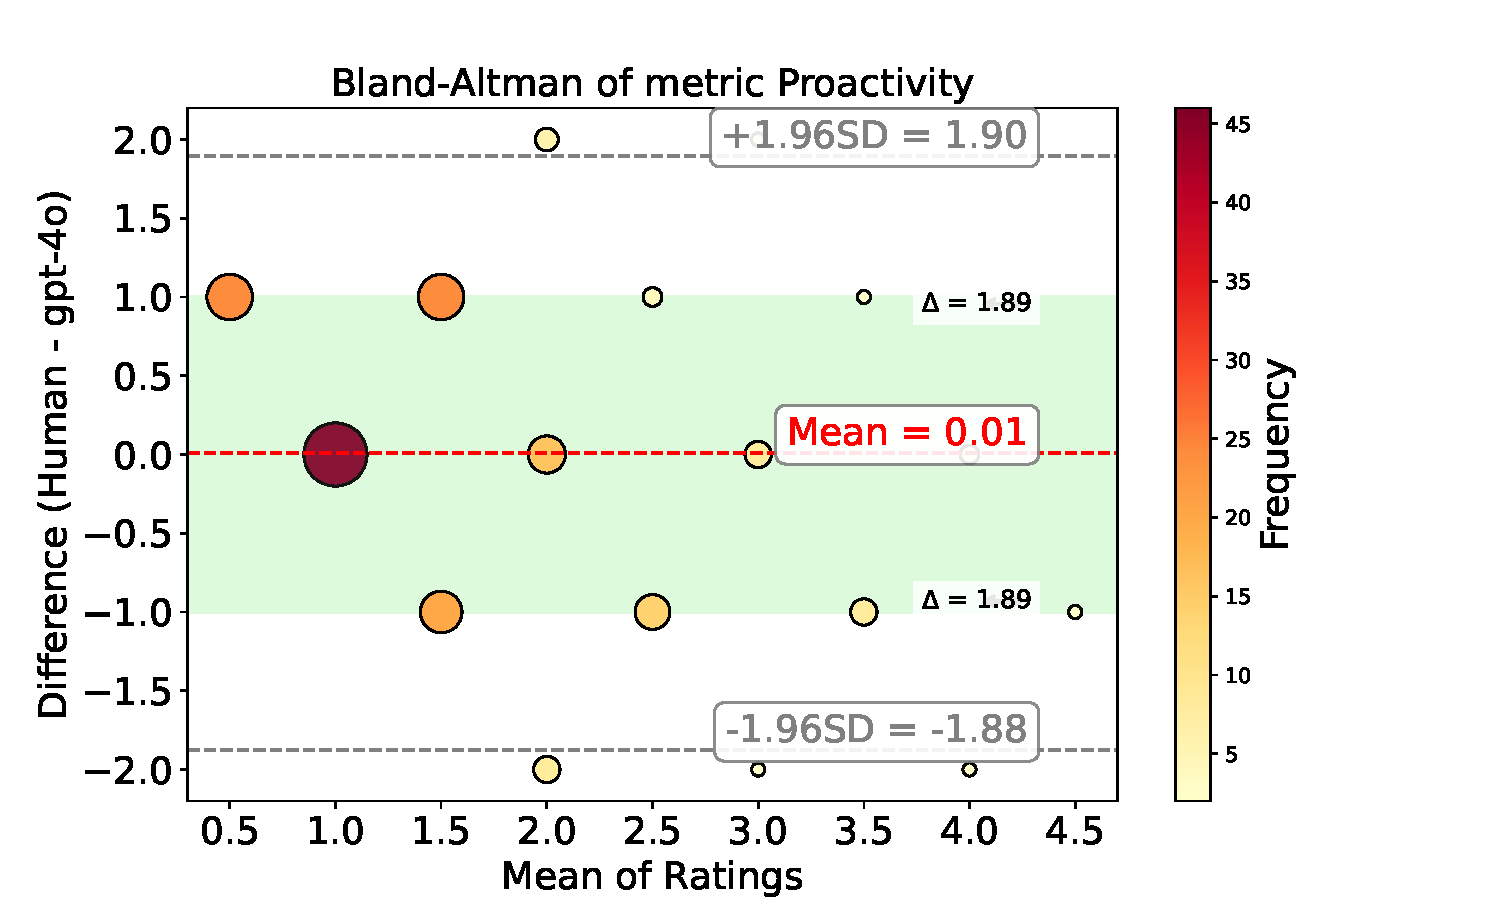
\includegraphics[width=\linewidth]{pic/Proactivity_human_gpt-4o-2024-11-20.pdf}
        \caption{提供 key points 时，\textbf{Proactivity} 指标的 Bland-Altman 分析结果。}
        \label{fig:w_keypointres_proactivity}
    \end{minipage}
    \hfill 
    \begin{minipage}[t]{0.48\textwidth}
        \centering
        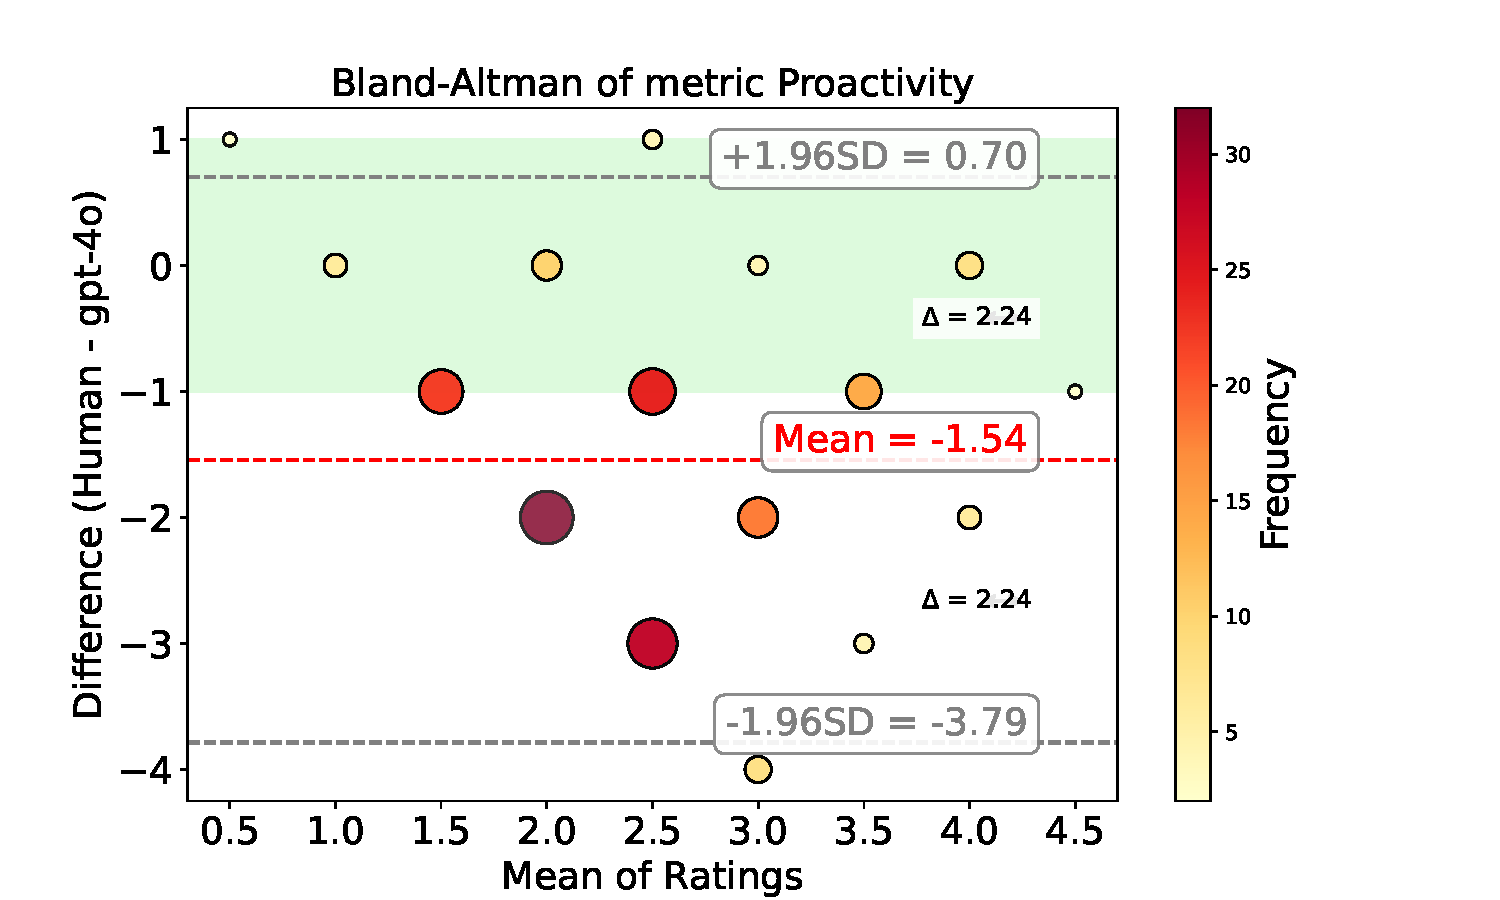
\includegraphics[width=\linewidth]{pic/Proactivity_human_gpt-4o-2024-11-20_wk.pdf}
        \caption{不提供 key points 时，\textbf{Proactivity} 指标的 Bland-Altman 分析结果。}
        \label{fig:wo_keypointres_proactivity}
    \end{minipage}
\end{figure*}



为了验证 key-point-based LLM evaluation 方法的有效性，我们针对 GPT-4o 模型，在 Tool-Given 与 Tool-Retrieval 两种设定下，为每种 method 各收集 16 个数据点，共计 96 个数据点。随后，我们分析其与人工评测的一致性，以验证该方法的有效性。
% z





为了量化一致性，我们采用 Bland-Altman method。该方法以两种测量值的平均值为横轴、二者差值为纵轴，并给出三条参考线：mean difference（红色虚线）以及 95\% limits of agreement（LoA），其计算方式为 mean ± 1.96 × standard deviation。如果大多数数据点落在 LoA 范围内，则说明两种方法具有良好一致性。点的大小表示样本数，绿色区域则标出分差不超过 1 分的样本。




Figure~\ref{fig:w_keypointres_proactivity} 与 Figure~\ref{fig:wo_keypointres_proactivity} 中关于 Proactivity 指标的实验结果表明：(1) System Bias Control：在 key-point constraint 下，mean difference 为 0.01（95\% CI: -1.88 $\sim$ 1.90），接近理论理想值 0，说明在总分维度上 LLM 评测与人工评测在统计意义上具有一致性。(2) LoA Interval Length：与自由评测模式相比，key-point constraint 缩小了 LoA 区间宽度（1.89 vs. 2.24）。(3) Error Distribution Characteristics：89.6\% 的样本分差不超过 1 分（绿色区域），相比不提供 key points 的对照组提升了超过 39.6 个百分点。
这些发现验证了 key-point-based LLM evaluation strategy 的有效性。更多细节请参见 Appendix~\ref{sec:appendix_effectiveness_of_key-point-based_LLM_evaluation}。




\section{Related Works}

\subsection{Personalization of LLM}
LLM 的个性化旨在与个体偏好对齐 \cite{zollo2025personalllm, tseng2024talespersonallmssurvey}。当前个性化任务通常聚焦于特定文本生成 \cite{he2025cosenhancingpersonalizationmitigating, zhao2025do, lee2024aligningthousandspreferencesmessage}、推荐任务 \cite{yang2023palrpersonalizationawarellms}、role-playing \cite{wang-etal-2024-rolellm, shao-etal-2023-character}、新闻标题生成 \cite{salemi-etal-2024-lamp}、对话任务，以及教育 \cite{Pratama2023REVOLUTIONIZINGEH} 与医疗 \cite{10.1145/3437963.3441657, abbasian2024conversationalhealthagentspersonalized} 等应用；其评测过程通常涉及从上下文中总结用户 preference 以生成响应 \cite{zhang2024guidedprofilegenerationimproves}。然而，Personal LLM Agents 更进一步，它定义了一种应当具备 interactive capabilities 的理想 personal assistant \cite{singh-etal-2024-personal}。我们提出 ETAPP，正是为了解决在多样化场景下，Personal LLM Agents 的评测缺乏 personalized tool usage 标准这一问题。









\subsection{Tool-augmented LLM}
Tool-augmented LLMs 旨在使模型能够通过工具与外部世界交互 \cite{10.1145/3704435, qu2025tool}。已有大量 benchmark 与方法被提出，用于评测并提升 tool utilization 与 task completion 的准确性 \cite{trivedi-etal-2024-appworld,li-etal-2023-api, hao2024citienhancingtoolutilizing, tang2023toolalpacageneralizedtoollearning, NEURIPS2023_9cb2a749}。然而，这些数据集主要面向一般人群，而非针对个体用户偏好定制的 personalized tool invocation。我们的工作将 tool invocation process 与 personalization 结合起来，并围绕这一目标提出相应的评测指标与方法。




\section{Conclusion}
本文评估了 large language models 在交互环境中提供个性化服务的能力与水平。我们将 tool invocation 过程与个性化服务结合起来，并提出两个评测指标：Personalization 与 Proactivity。为解决在该任务中使用 LLM 作为 evaluator 所带来的不可靠性问题，我们引入了一种基于 key point 的 LLM evaluation 方法，并验证了其可靠性。最后，我们分析了不同模型在该任务上的表现，并探讨了提升其个性化 tool utilization 能力所面临的挑战与可能方向。

\section*{Limitations}
我们从 personalization 与 proactivity 的视角评估了 LLM 中 tool utilization 的个性化，并提出了一种基于 key point 的 LLM evaluation 方法。然而，该方向仍存在若干挑战。例如，我们的工作尚未考虑 multimodal tasks；同时，也还有一些细节可以进一步细化。例如，在 preference modeling 过程中，我们还可以进一步建模用户对相似工具的选择偏好（例如当两个应用 A 和 B 提供相同功能时，用户可能更倾向于使用 App A 的 API 来完成任务）。未来我们计划将这项工作扩展到多模态领域。

\section*{Ethics Statement}
我们的工作不引入额外伦理问题。本文在稿件语言润色过程中使用了 AI assistance，包括词汇修正与拼写检查。


% Bibliography entries for the entire Anthology, followed by custom entries
%\bibliography{anthology,custom}
% Custom bibliography entries only
\bibliography{custom}
\newpage
\appendix


\section{数据集构建}
\label{sec:dataset_construction}

\subsection{工具构建}
我们构建的工具列于 Table~\ref{table:api_name}。大多数工具的输出都由真实世界 API 数据生成。例如，weather data 来自 WeatherAPI.com \footnote{https://rapidapi.com/weatherapi/api/weatherapi-com}，music data 来自 Genius - Song Lyrics \footnote{https://rapidapi.com/Glavier/api/genius-song-lyrics1}，shopping products 则来自 RapidAPI 中的 Real-Time Amazon Data \footnote{https://rapidapi.com/letscrape-6bRBa3QguO5/api/real-time-amazon-data}。Navigation data 则由同样来源于真实世界数据的 TravelPlanner \cite{xie2024travelplanner} 修改而来。我们调整了记录日期，并加入了数十条由 gpt-4o 生成的数据。News data 则完全由 gpt-4o 生成。

\subsection{用户偏好}
我们在 benchmark 中构建了 16 位用户，每位用户都具有一个 User Profile 和 Tool-utilizing Preference。

User Profile 的示例见 Example~\ref{Example:User_Profile}。Tool-utilizing Preference 的示例见 Example~\ref{Example:Tool_utilizing_Preference}。用户 \textit{James Harrington} 在 API \textit{get\_user\_recent\_workout\_records} 上的一条 interaction history 示例见 Example~\ref{Example:Interaction_History}。



\subsection{Interaction History 构建流程}
\label{sec:appendix_instruction_history}
为了保证 interaction history 的一致性，我们首先为每位用户构建一个 9 天安排，并在此基础上构造 interaction history，内容覆盖 schedule arrangements、alarms、health status（按小时更新）、exercise records、email records 与 music collections。interaction history 的具体构建步骤如下：(1) 基于 user profile 生成用户的 9 天 schedule；(2) 对 schedule 进行细化扩展；(3) 根据 user profile 与 schedule 生成对应的 interaction history；(4) 进行人工核验以确保一致性与准确性。

\subsection{Key Points 标注}
对于人工标注的 key points，我们由两位研究生共同完成标注与核验，以尽可能保证其全面性与可靠性。

\section{评测细节}
\label{sec:evaluation_details}

\subsection{Tool-invoking Method}
Tool-Given 与 Tool-Retrieval 设定下，FC、ReAct 和 E-ReAct 格式的 tool-invoking prompt 分别见 Prompt~\ref{Prompt:ReAct_Tool_Given}、Prompt~\ref{Prompt:FC_Tool_Given}、Prompt~\ref{Prompt:E-ReAct_Tool_Given}、Prompt~\ref{Prompt:ReAct_Tool_Retrieval}、Prompt~\ref{Prompt:FC_Tool_Retrieval} 和 Prompt~\ref{Prompt:E-ReAct_Tool_Retrieval}。其中 ``\{'' 与 ``\}'' 中的内容会在 inference 过程中被替换为具体内容。





\subsection{实现细节}
在两种实验设定下，我们使用以下具备 function calling 能力的模型作为 baselines：gpt-4o-2024-11-20、DeepSeek-V3 \cite{deepseekai2024deepseekv3technicalreport}、Qwen2.5-72B-Instruct \cite{qwen2.5}、Llama-3.1-70B-Instruct \footnote{https://huggingface.co/meta-llama/Llama-3.1-70B-Instruct}，以及 watt-tool-70B \footnote{https://huggingface.co/watt-ai/watt-tool-70B}（BFCL 中表现最好的模型）。此外，由于 budget 因素，我们还在 100 条测试数据的子集上，使用 ReAct method 评测了 reasoning model：o1-preview-2024-09-12、o1-mini-2024-09-12、DeepSeek-R1 \cite{deepseekai2025deepseekr1incentivizingreasoningcapability}、DeepSeek-R1-Distill-Qwen-32B \cite{deepseekai2025deepseekr1incentivizingreasoningcapability} 和 QwQ-32B-Preview \cite{qwq-32b-preview}；这些模型均不支持 FC。



对于 reasoning model，在我们的实验中，其 reasoning content 不被计入 tool-invoking process。

对于 fine-tuning experiments，我们使用 LoRA 对模型进行微调。其中 rank $r$ 设为 8，lora alpha 设为 16；epoch 设为 3，learning rate 设为 1e-4，batch size 设为 32。数据采用 interaction format，我们将每个带有 API 的 interaction turn 划分为训练数据，最终将标注的 200 条 instructions 划分为 841 条训练样本。实验在 NVIDIA A100 上完成。

\subsection{评测 Prompt}
key-point-based LLM Evaluation 的 Prompt 见 Prompt~\ref{Prompt:Key_Point_Evaluation}。其中 ``\{'' 与 ``\}'' 中的内容会在 evaluation 过程中被替换为具体内容。由 GPT-4o 生成的一条 evaluation output 示例见 Example~\ref{Example:Evaluation_Result_Example}。

\subsection{错误示例}
\label{sec:appendix_example_error}
一些错误示例见 Example~\ref{Example:Example_of_Error}。

\section{key-point-based LLM evaluation 的有效性}

\label{sec:appendix_effectiveness_of_key-point-based_LLM_evaluation}
Procedure 与 Personalization 两个指标的 Bland-Altman 分析结果见 Figure~\ref{fig:w_keypointres_procedure}、Figure~\ref{fig:wo_keypoint_res_procedure}、Figure~\ref{fig:w_keypoint_res_personalization} 和 Figure~\ref{fig:wo_keypoint_res_personalization}。我们观察到，key points 在提升 Personalization 与 Proactivity 指标评测过程的一致性方面起到了关键作用。尽管 evaluation model 已经获得了评分标准，但即使没有 key points，它也倾向于给出较高分。我们认为，这可能是因为模型对“assistant 应如何提供个性化且主动的服务”缺乏充分知识和理解。一旦输入 key points，evaluation model 就能够逐点分析每个要求是否被满足，从而提升最终分析质量与评分准确性。不过我们也注意到，在 Procedure 指标上，加入 key points 后 mean difference 反而更差。这可能是因为三个指标是同时评测的，而 Procedure 会受到另外两个指标的影响，因此整体得分被拉低。





\begin{table*}
{
    \centering
    \resizebox{1\textwidth}{!}{
    \begin{tabular}{c|c}
         % &  \\
         \toprule
         Category & API Name \\
         \midrule
         HealthMonitoringApp & get\_current\_health\_and\_mood\_status \\
HealthMonitoringApp & get\_user\_recent\_workout\_records \\
HealthMonitoringApp & get\_recent\_health\_and\_mood\_summary \\
Calendar & add\_event\_in\_calendar \\
Calendar & view\_today\_events\_in\_calendar \\
Calendar & view\_events\_in\_calendar\_by\_providing\_time\_range \\
Calendar & delete\_event\_in\_calendar \\
Calendar & add\_alarm \\
Calendar & view\_today\_alarms \\
WeatherData & get\_today\_weather \\
WeatherData & get\_future\_weather \\
ECommerce & add\_product\_to\_cart \\
ECommerce & search\_products\_in\_shopping\_manager \\
ECommerce & view\_cart\_in\_shopping\_manager \\
Email & send\_email \\
Email & get\_today\_emails\_until\_now \\
Email & search\_email\_by\_sender\_and\_receiver \\
Email & search\_email\_by\_content \\
Browser & search\_news\_by\_category \\
Browser & search\_heat\_news \\
Browser & search\_from\_wikipedia \\
MusicStreamingApp & play\_music \\
MusicStreamingApp & get\_music\_list\_in\_favorites \\

Navigation\_And\_Map & find\_accommodations \\
Navigation\_And\_Map & find\_attractions \\
Navigation\_And\_Map & find\_restaurants \\
Navigation\_And\_Map & find\_flight \\
Thermostat (Smart\_Home\_Devices) & set\_temperature\_and\_humidity\_in\_home \\
Thermostat (Smart\_Home\_Devices) & get\_home\_temperature\_and\_humidity \\
Light (Smart\_Home\_Devices) & control\_light\_in\_home \\
SmartAppliance (Smart\_Home\_Devices) & control\_curtains\_in\_home \\
SmartAppliance (Smart\_Home\_Devices) & control\_bathtub\_in\_home \\
SmartAppliance (Smart\_Home\_Devices) & boil\_water\_in\_home \\
\midrule
Tool\_Searcher & search\_tools \\
Tool\_Searcher & get\_tool\_doc \\
\midrule
    \end{tabular}
    }
}
    \caption{API 及其对应类别信息。}
    \label{table:api_name}
\end{table*}


\begin{table*}[]
    \centering
    \begin{tabular}{c|c}
        \toprule
        Statistics & Number \\
        \toprule
        Tool Categories & 9 \\
        APIs Number & 35 \\
        Instruction Number & 800 \\
        User Number & 16 \\
        Key points Number of Personalization per query & 3.18 \\
        Key points Number of Proactivity per query & 3.2 \\
        Avg. Turns per query  & 3.43 \\
        \midrule
    \end{tabular}
    \caption{ETAPP 的统计信息。Avg. Turn 基于 GPT-4o 在 Tool-Given 设定、ReAct 格式下的输出计算得到。}
    \label{table:statistics}
\end{table*}



\begin{figure*}[htbp]
    \centering
    \begin{minipage}[t]{0.48\textwidth}
        \centering
        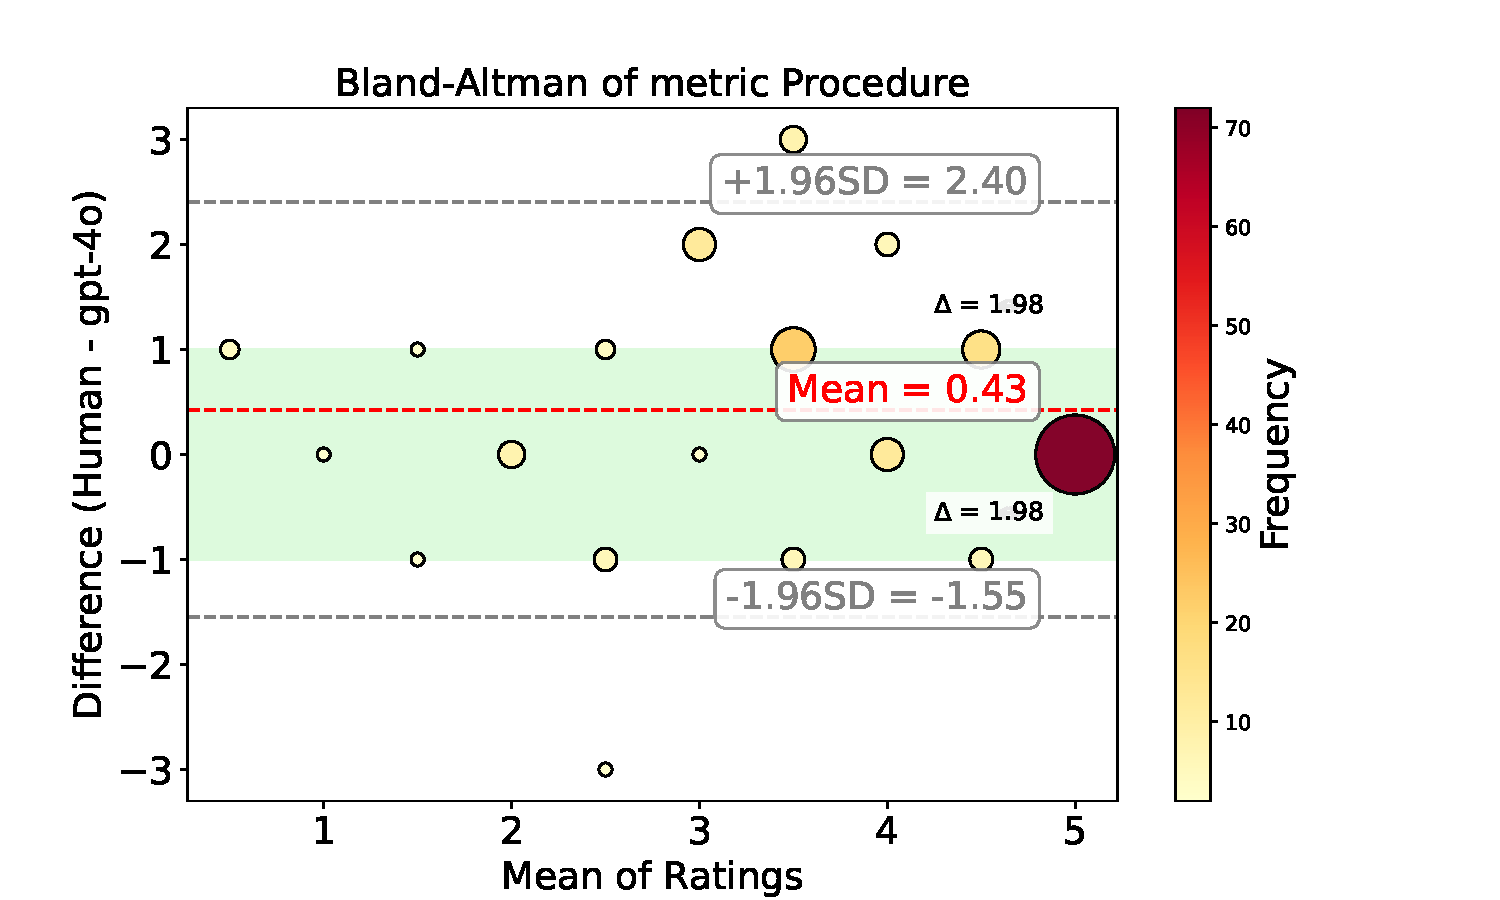
\includegraphics[width=\linewidth]{pic/Procedure_human_gpt-4o-2024-11-20.pdf}
        \caption{提供 key points 时，\textbf{Procedure} 指标的 Bland-Altman 分析结果。}
        \label{fig:w_keypointres_procedure}
    \end{minipage}
    \hfill % 添加一些水平间距
    \begin{minipage}[t]{0.48\textwidth}
        \centering
        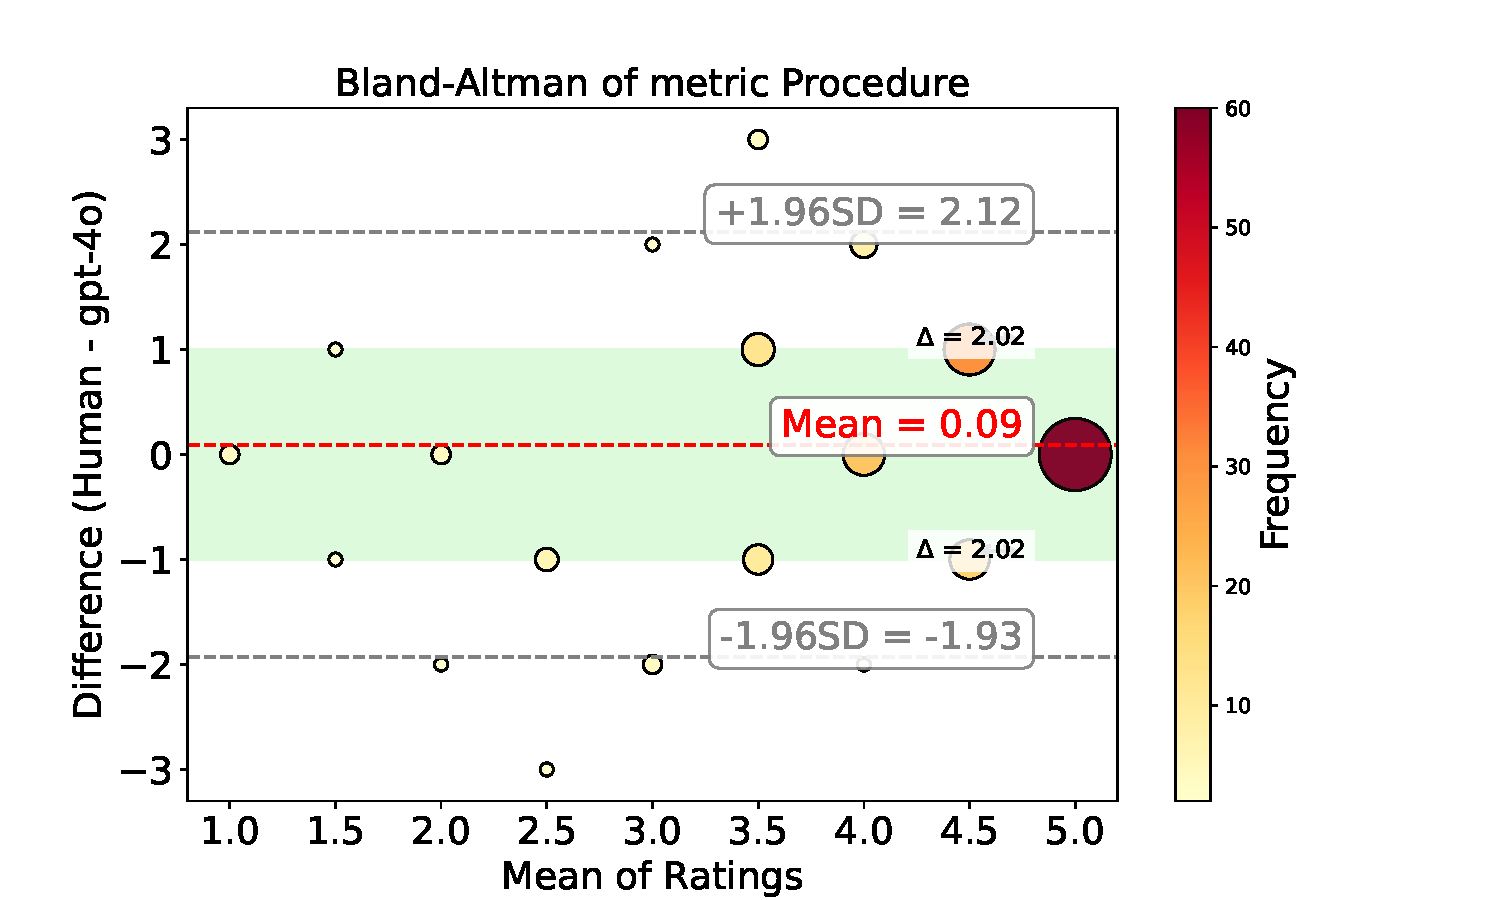
\includegraphics[width=\linewidth]{pic/Procedure_human_gpt-4o-2024-11-20_wk.pdf}
        \caption{不提供 key points 时，\textbf{Procedure} 指标的 Bland-Altman 分析结果。}
        \label{fig:wo_keypoint_res_procedure}
    \end{minipage}
\end{figure*}

\begin{figure*}[htbp]
    \centering
    \begin{minipage}[t]{0.48\textwidth}
        \centering
        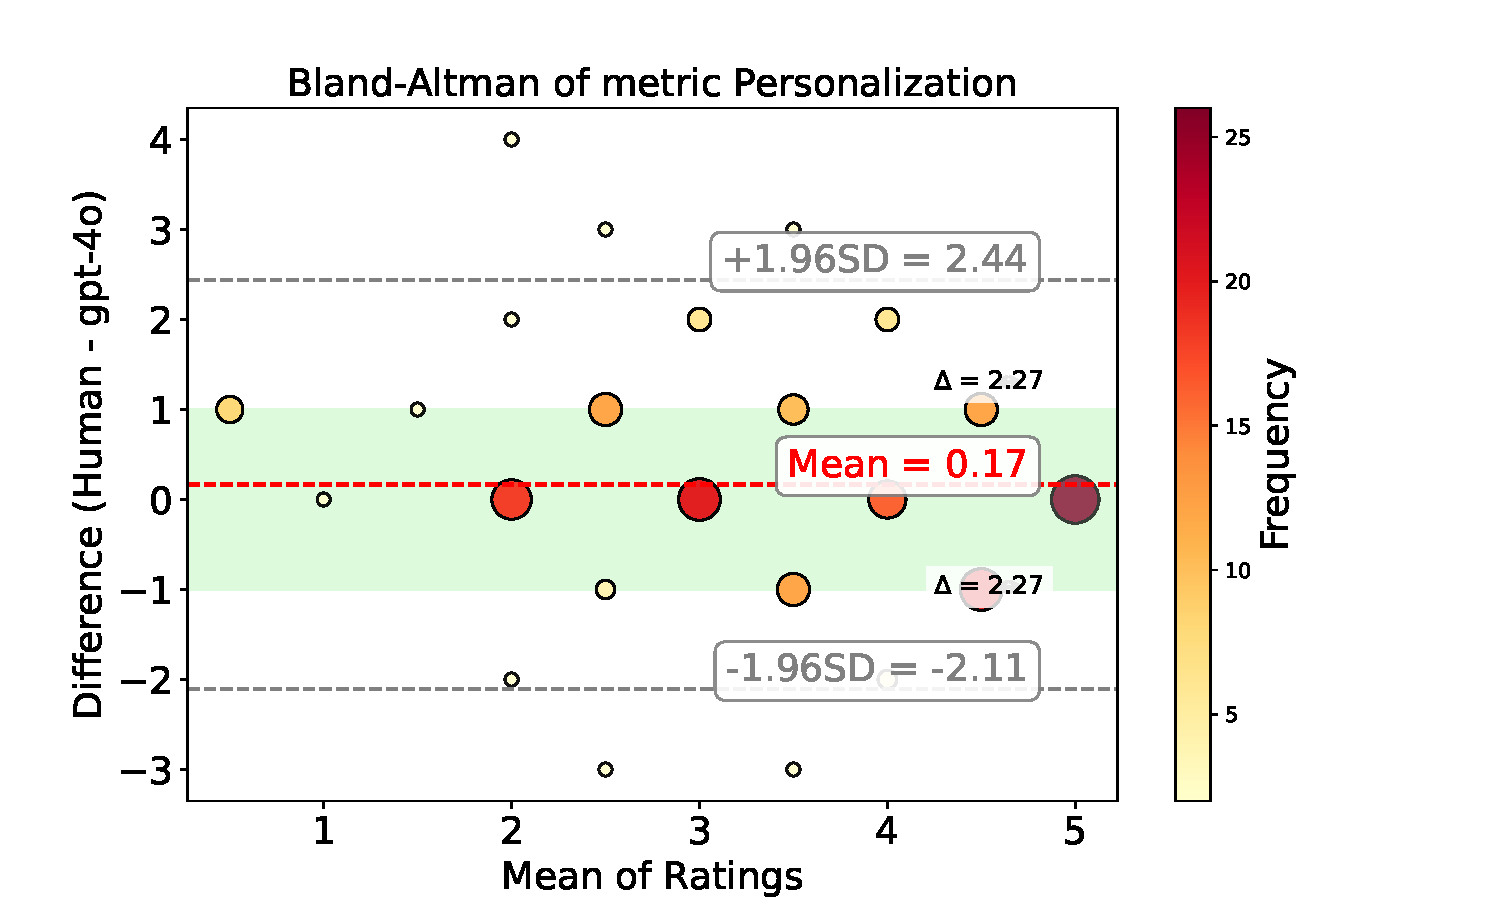
\includegraphics[width=\linewidth]{pic/Personalization_human_gpt-4o-2024-11-20.pdf}
        \caption{提供 key points 时，\textbf{Personalization} 指标的 Bland-Altman 分析结果。}
        \label{fig:w_keypoint_res_personalization}
    \end{minipage}
    \hfill % 添加一些水平间距
    \begin{minipage}[t]{0.48\textwidth}
        \centering
        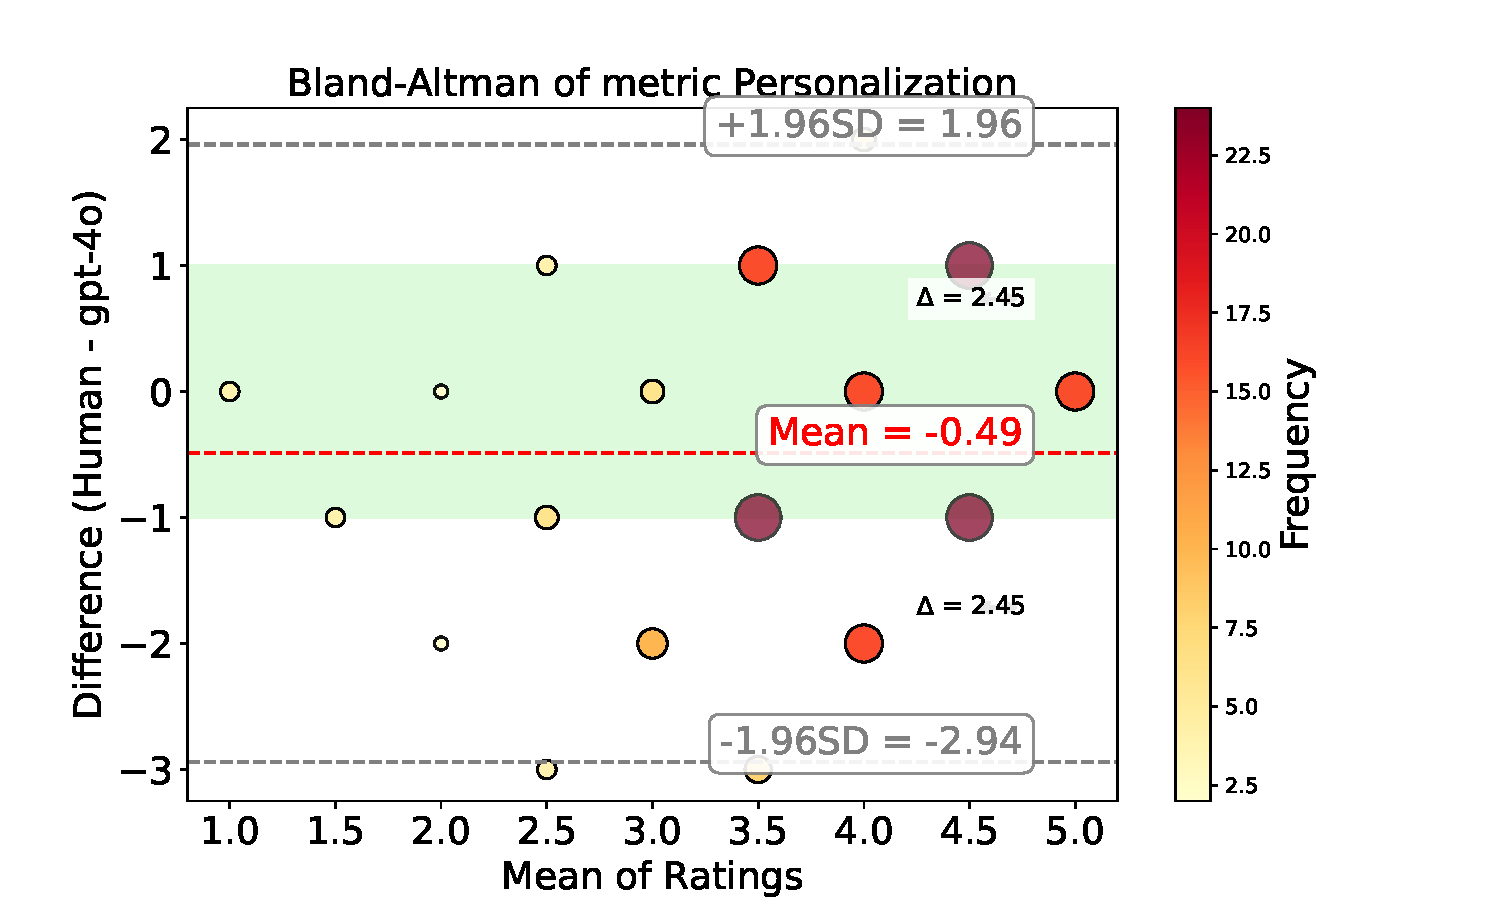
\includegraphics[width=\linewidth]{pic/Personalization_human_gpt-4o-2024-11-20_wk.pdf}
        \caption{不提供 key points 时，\textbf{Personalization} 指标的 Bland-Altman 分析结果。}
        \label{fig:wo_keypoint_res_personalization}
    \end{minipage}
\end{figure*}






\newpage
\onecolumn
\begin{tcolorbox}[width=\textwidth, breakable]
{

\renewcommand{\lstlistingname}{Example}

\lstinputlisting[frame=none, basicstyle=\ttfamily\footnotesize, breaklines=true, columns=fullflexible, postbreak=\mbox{\textcolor{red}{$\hookrightarrow$}\space},
    breakatwhitespace=true, label=Example:User_Profile, caption=User Profile 示例, captionpos=b, ]{./profile.txt}
}




\end{tcolorbox}

\begin{tcolorbox}[width=\textwidth, breakable,]
{
\renewcommand{\lstlistingname}{Example}

\lstinputlisting[frame=none, basicstyle=\ttfamily\footnotesize, breaklines=true, columns=fullflexible, postbreak=\mbox{\textcolor{red}{$\hookrightarrow$}\space},
    breakatwhitespace=true, label=Example:Tool_utilizing_Preference, caption=Tool-utilizing Preference 示例, captionpos=b, ]{./tool-utilizing_preference.txt}
}





\end{tcolorbox}

\begin{tcolorbox}[width=\textwidth, breakable, ]
{
\renewcommand{\lstlistingname}{Example}
% \label{Example:Interaction_History}
\lstinputlisting[frame=none, basicstyle=\ttfamily\footnotesize, breaklines=true, columns=fullflexible, postbreak=\mbox{\textcolor{red}{$\hookrightarrow$}\space},
    breakatwhitespace=true, label=Example:Interaction_History, caption=Interaction History 示例, captionpos=b, ]{./Interaction_History.txt}
}





\end{tcolorbox}
\begin{tcolorbox}[width=\textwidth, breakable, ]
{
\renewcommand{\lstlistingname}{Example}
% \label{Example:User_Profile}
\lstinputlisting[frame=none, basicstyle=\ttfamily\footnotesize, breaklines=true, columns=fullflexible, postbreak=\mbox{\textcolor{red}{$\hookrightarrow$}\space},
    breakatwhitespace=true, label=Example:Example_of_Error, caption=错误输出示例, captionpos=b, ]{./Example_Error.txt}
}



\end{tcolorbox}



\newpage
% \onecolumn
\begin{tcolorbox}[width=\textwidth, breakable, ]
{
\renewcommand{\lstlistingname}{Prompt}
% \label{Prompt:ReAct_Tool_Given}
\lstinputlisting[frame=none, basicstyle=\ttfamily\footnotesize, breaklines=true, columns=fullflexible, postbreak=\mbox{\textcolor{red}{$\hookrightarrow$}\space}, % Indicate line breaks% basicstyle=\ttfamily,    % Use monospaced font
    breakatwhitespace=true, label=Prompt:ReAct_Tool_Given, caption=ReAct（Tool-Given）, captionpos=b, ]{./Prompt_Template_ReAct_Tool_Given.txt}
}


\end{tcolorbox}



\begin{tcolorbox}[width=\textwidth, breakable, ]
{
\renewcommand{\lstlistingname}{Prompt}
% \label{Prompt:FC_Tool_Given}
\lstinputlisting[frame=none, basicstyle=\ttfamily\footnotesize, breaklines=true, columns=fullflexible, postbreak=\mbox{\textcolor{red}{$\hookrightarrow$}\space}, % Indicate line breaks% basicstyle=\ttfamily,    % Use monospaced font
    breakatwhitespace=true, label=Prompt:FC_Tool_Given, caption=FC（Tool-Given）, captionpos=b,]{./Prompt_Template_FC_Tool_Given.txt}
}


\end{tcolorbox}

% \onecolumn
\begin{tcolorbox}[width=\textwidth, breakable, ]
{
\renewcommand{\lstlistingname}{Prompt}
% \label{Prompt:E-ReAct_Tool_Given}
\lstinputlisting[frame=none, basicstyle=\ttfamily\footnotesize, breaklines=true, columns=fullflexible, postbreak=\mbox{\textcolor{red}{$\hookrightarrow$}\space}, % Indicate line breaks% basicstyle=\ttfamily,    % Use monospaced font
    breakatwhitespace=true, label=Prompt:E-ReAct_Tool_Given, caption=E-ReAct（Tool-Given）, captionpos=b,]{./Prompt_Template_E-ReAct_Tool_Given.txt}
}


\end{tcolorbox}


% \onecolumn
\begin{tcolorbox}[width=\textwidth, breakable, ]
{
\renewcommand{\lstlistingname}{Prompt}
% \label{Prompt:ReAct_Tool_Retrieval}
\lstinputlisting[frame=none, basicstyle=\ttfamily\footnotesize, breaklines=true, columns=fullflexible, postbreak=\mbox{\textcolor{red}{$\hookrightarrow$}\space}, % Indicate line breaks% basicstyle=\ttfamily,    % Use monospaced font
    breakatwhitespace=true, label=Prompt:ReAct_Tool_Retrieval, caption=ReAct（Tool-Retrieval）, captionpos=b,]{./Prompt_Template_ReAct_Tool_Retrieval.txt}
}

\end{tcolorbox}


% \onecolumn
\begin{tcolorbox}[width=\textwidth, breakable, ] % (Tool-Retrieval)
{
\renewcommand{\lstlistingname}{Prompt}
% \label{Prompt:FC_Tool_Retrieval}
\lstinputlisting[frame=none, basicstyle=\ttfamily\footnotesize, breaklines=true, columns=fullflexible, postbreak=\mbox{\textcolor{red}{$\hookrightarrow$}\space}, % Indicate line breaks% basicstyle=\ttfamily,    % Use monospaced font
    breakatwhitespace=true, label=Prompt:FC_Tool_Retrieval, caption=FC（Tool-Retrieval）, captionpos=b,]{./Prompt_Template_FC_Tool_Retrieval.txt}
}

\end{tcolorbox}


% \onecolumn
\begin{tcolorbox}[width=\textwidth, breakable, ]
{
\renewcommand{\lstlistingname}{Prompt}
% \label{Prompt:E-ReAct_Tool_Retrieval}
\lstinputlisting[frame=none, basicstyle=\ttfamily\footnotesize, breaklines=true, columns=fullflexible, postbreak=\mbox{\textcolor{red}{$\hookrightarrow$}\space}, % Indicate line breaks% basicstyle=\ttfamily,    % Use monospaced font
    breakatwhitespace=true, label=Prompt:E-ReAct_Tool_Retrieval, caption=E-ReAct（Tool-Retrieval）, captionpos=b,]{./Prompt_Template_E-ReAct_Tool_Retrieval.txt}
}



\end{tcolorbox}


% \onecolumn
\begin{tcolorbox}[width=\textwidth, breakable, ]
{
\renewcommand{\lstlistingname}{Prompt}
% \label{Prompt:Key_Point_Evaluation}
\lstinputlisting[frame=none, basicstyle=\ttfamily\footnotesize, breaklines=true, columns=fullflexible, postbreak=\mbox{\textcolor{red}{$\hookrightarrow$}\space},
    breakatwhitespace=true, label=Prompt:Key_Point_Evaluation, caption=key-point-based LLM Evaluation 的评测 Prompt, captionpos=b,]{./Prompt_evaluation.txt}
}



\end{tcolorbox}


% \onecolumn
\begin{tcolorbox}[width=\textwidth, breakable, ]
{
\renewcommand{\lstlistingname}{Example}
% \label{Example:Evaluation_Result_Example}
\lstinputlisting[frame=none, basicstyle=\ttfamily\footnotesize, breaklines=true, columns=fullflexible, postbreak=\mbox{\textcolor{red}{$\hookrightarrow$}\space},
    breakatwhitespace=true, label=Example:Evaluation_Result_Example, caption=评测结果示例, captionpos=b,]{./Evaluation_Result_Example.txt}
}



\end{tcolorbox}







\end{document}
